
%%%%%%%%%%%%%%%%%%%%%%%%%%%%%%%%%%%%%%%%%%%%%%%%%%%%%%%%%%%%%%%%%%%%%%%%%%%%%%%
%
%  EGSnrc getting started manual
%  Copyright (C) 2017 National Research Council Canada
%
%  This file is part of EGSnrc.
%
%  EGSnrc is free software: you can redistribute it and/or modify it under
%  the terms of the GNU Affero General Public License as published by the
%  Free Software Foundation, either version 3 of the License, or (at your
%  option) any later version.
%
%  EGSnrc is distributed in the hope that it will be useful, but WITHOUT ANY
%  WARRANTY; without even the implied warranty of MERCHANTABILITY or FITNESS
%  FOR A PARTICULAR PURPOSE.  See the GNU Affero General Public License for
%  more details.
%
%  You should have received a copy of the GNU Affero General Public License
%  along with EGSnrc. If not, see <http://www.gnu.org/licenses/>.
%
%%%%%%%%%%%%%%%%%%%%%%%%%%%%%%%%%%%%%%%%%%%%%%%%%%%%%%%%%%%%%%%%%%%%%%%%%%%%%%%
%
%  Authors:         Reid Townson
%                   Frederic Tessier
%                   Ernesto Mainegra-Hing
%
%  Contributors:
%
%%%%%%%%%%%%%%%%%%%%%%%%%%%%%%%%%%%%%%%%%%%%%%%%%%%%%%%%%%%%%%%%%%%%%%%%%%%%%%%


\documentclass[12pt,twoside]{article}
\setlength{\textwidth}{6.5in}
\setlength{\textheight}{9.3in}
\setlength{\oddsidemargin}{0.0in}
\setlength{\evensidemargin}{0.0in}
\setlength{\topmargin}{-0.6in}
\setlength{\parindent}{1.5em}
\setlength{\topsep}{0ex}
\setlength{\itemsep}{0ex}

\newcommand{\parsp}{~\hspace*{1.5em}}
\setlength{\parskip}{0.1in}
\setlength{\baselineskip}{0.4in}
\newcommand{\head}[1]{\begin{center}\begin{Large}{\bf #1}
                                              \end{Large}\end{center}}
\newcommand{\cen}[1]{\begin{center} #1 \end{center}                   }
\newcommand{\etal}{{\em et.al.}}
\newcommand{\etc}{{\em etc}}
\newcommand{\eg}{{\em e.g.}}
\newcommand{\ie}{{\em i.e.}}

\usepackage{hyperref}
\hypersetup{colorlinks=true, citecolor=blue, linkcolor=blue, filecolor=blue, urlcolor=blue}
\urlstyle{same}

\usepackage{float}
\usepackage{amsmath}
\usepackage{graphicx}
\usepackage{html}
\usepackage{fancyhdr}
\usepackage{multirow}
\usepackage{hhline}
\renewcommand{\footrulewidth}{0.4pt}
\renewcommand{\headrulewidth}{0.4pt}
\setlength{\headheight}{16pt}

%\lhead[{\sffamily \thepage~}]{{\sf NRCC Report PIRS-EGS-101}}
\rhead[{\sf Getting Started with EGSnrc}]{{\sffamily ~\thepage}}
\rfoot{{{\sf \rightmark}}}
%\lfoot[{{\sf \leftmark}}]{{\small Last edited Date: 2018/03/20}}
\cfoot{}

\renewcommand{\refname}{}

% ====================================
% These settings are from EGSnrc labs
\usepackage{fancyvrb}

\usepackage{color}
\definecolor{white}{rgb}{1,1,1}
\definecolor{gray}{rgb}{0.6,0.6,0.6}
\definecolor{red}{rgb}{0.85,0,0}
\definecolor{green}{rgb}{0,0.85,0}
\definecolor{blue}{rgb}{0,0,1}
\definecolor{verb}{cmyk}{1,0.2,0,0.2}
\definecolor{beige}{rgb}{0.92,0.87,0.78}
\definecolor{question}{rgb}{0.1,0.6,0.1}

%% code listings
\usepackage{listings}
\definecolor{terminal}{rgb}{0.91,0.96,0.91}
\definecolor{rule}{rgb}{0.3,0.4,0.3}
\definecolor{prompt}{rgb}{0.6,0.7,0.6}
\definecolor{keyword}{cmyk}{1,0.2,0,0.2}
\definecolor{comment}{rgb}{0.6,0,0}

\lstset{
    language=bash,
    aboveskip=2ex,
    frame=single,
    framerule=0.4pt,
    rulecolor=\color{rule},
    framesep=6pt,
    framexleftmargin=5pt,
    xleftmargin=10pt,
    xrightmargin=5pt,
    framextopmargin=2pt,
    backgroundcolor=\color{terminal},
    basicstyle=\ttfamily,
    breaklines=true,
    postbreak=\mbox{\textcolor{red}{$\hookrightarrow$}\space},
    commentstyle=\color{comment},
    classoffset=0,
    keywordstyle=\color{keyword},
    classoffset=1,
    morekeywords={\$},keywordstyle=\color{prompt},
    classoffset=0
}

\fvset{formatcom=\color{verb}}

\raggedbottom

% --------------------------------------------------------------------------------
% Question environment
% --------------------------------------------------------------------------------
\makeatletter
% question counter and label
\@definecounter{questi}
\renewcommand\thequesti         {\@arabic\c@questi}
\newcommand\labelquesti         {\thequesti}
\newsavebox\questbox


% question environment
\newenvironment{question}{
    \bfseries
    \edef\@questictr{questi}
    \expandafter
    \list \csname label\@questictr\endcsname {
        \usecounter\@questictr\def\makelabel##1{\hss\llap{##1}}
        \savebox{\questbox}             {\thequesti}
        \setlength\labelsep             {0.6em}
        \setlength\labelwidth           {\wd\questbox}
        \setlength\leftmargini          {\labelwidth}
        \addtolength{\leftmargini}      {\labelsep}
        \addtolength{\leftmargini}      {0.2em}
        \leftmargin\leftmargini
        \setlength\topsep               {1em}
        \setlength\itemsep              {1.2em}
        \setlength\parsep               {0.5em}
    }
}{\normalfont\endlist}

\makeatother

% answer
\newenvironment{answer}{\normalfont}{\relax}

% scientific notation shorthand
\providecommand{\e}[1]{\ensuremath{\times 10^{#1}}}

% ====================================

\begin{document}

\thispagestyle{empty}

% Make it so lstlisting can be copy/pasted from
\lstset{basicstyle = \ttfamily,columns=fullflexible}

\begin{htmlonly}
For information about the authors and/or institutions involved with this
work, use the links provided in the author list.
\begin{rawhtml}
<br><br>
\end{rawhtml}

\begin{rawhtml}
<br><br>
\end{rawhtml}

\begin{rawhtml}
<br><br>
\end{rawhtml}

Use the Up button to get back to this page from within the document.
\begin{rawhtml}
<BR> <HR> <P>
\end{rawhtml}
\copyright
Copyright 2017, National Research Council of Canada Ottawa
\begin{rawhtml}
<BR> <HR> <P>
\end{rawhtml}
\end{htmlonly}

%\setcounter{page}{1}
\pagestyle{empty}

\title{Getting Started with EGSnrc}
\author{ R. Townson, F. Tessier, E. Mainegra, B. Walters \\
Ionizing Radiation Standards\\
National Research Council of Canada,
Ottawa\\
}

\date{Printed: \today \\
%NRCC Report PIRS-EGS-101
\begin{latexonly}
\end{latexonly}
}
\maketitle

\pagenumbering{arabic}
\setlength{\parindent}{0em}

\begin{center}
\begin{Large}
{\bf Abstract}
\end{Large}
\end{center}
This manual is a ``quick start'' guide to help new users get familiar with EGSnrc. A number of complete tutorials are presented along with general guidance intended both for new users and for those looking to update their EGSnrc skills. It is suggested that the reader follows the document from top to bottom, as concepts are introduced gradually and through applied examples. The expected outcome is to provide the reader with some practical skills, along with a broader understanding of the capabilities of EGSnrc and the included tools. However, the information provided here is not complete: it will be necessary to refer to the relevant manuals for full technical descriptions.

\newpage
\mbox{}	%blank behind title page
\newpage
\setcounter{page}{1}
\pagestyle{fancy}

\tableofcontents

\newpage

%\pagestyle{myheadings}

\section{What is EGSnrc?}
EGSnrc is a software toolkit used to perform Monte Carlo simulation of
ionizing radiation transport through matter. It models the propagation
of photons, electrons and positrons with kinetic energies between
1~keV and 10~GeV, in homogeneous materials. EGSnrc is an
extended and improved version of the Electron Gamma Shower (EGS)
software package originally developed at the Stanford Linear Accelerator
Center (SLAC) in the 1970s. Most notably, it incorporates significant
refinements in charged particle transport, better low energy cross
sections, and the egs++ class library to model elaborate geometries and
particle sources.

EGSnrc is distributed with a wide range of applications (previously referred to
as ``user codes'') that utilize the radiation transport physics to calculate
specific quantities. These codes have been developed by numerous authors over
the lifetime of EGSnrc to support the large user community. For a brief
description of each application, see section \ref{apps}.

\section{Installation}

For the most up-to-date installation instructions, see the wiki section of the
EGSnrc github page:

\href{https://github.com/nrc-cnrc/EGSnrc/wiki/Installation-overview}{https://github.com/nrc-cnrc/EGSnrc/wiki/Installation-overview}


If you have any issues with the installation process, the EGSnrc reddit community is a good place to seek support:

\href{https://www.reddit.com/r/EGSnrc/}{https://www.reddit.com/r/EGSnrc/}

\addtocontents{toc}{\protect\setcounter{tocdepth}{2}}
% From this point on, only show up to \subsection in the ToC


\clearpage
\section{EGSnrc overview: the applications}
\label{apps}

\addtocontents{toc}{\protect\setcounter{tocdepth}{3}}
% From this point on, only show up to \subsubsection in the ToC

\begin{itemize}
\item EGSnrc is a collection of generic routines that simulate the transport
and interactions of photons, electrons and positrons in matter.
\item The majority of users do not write their own applications - the codes distributed
with EGSnrc are useful for a wide range of calculations.
\item Users can write their own applications that take advantage of the EGSnrc
system, or \textit{toolkit}, by writing a program which specifies their
particular problem in the \Verb+MAIN+ program and communicates with EGSnrc
through the user-supplied routines \Verb+AUSGAB+, \Verb+HOWFAR+ and \Verb+HOWNEAR+
and the EGSnrc routines \Verb+HATCH+ and \Verb+SHOWER+.
\item In principle, applications can be written in any programming language as
long as it can interface with the Fortran EGSnrc code-base.
\item Most commonly, applications are written in \Verb+MORTRAN3+ (native EGSnrc
language) or C++, although they could also be written in \Verb+FORTRAN+ or C.
\end{itemize}

\begin{center}
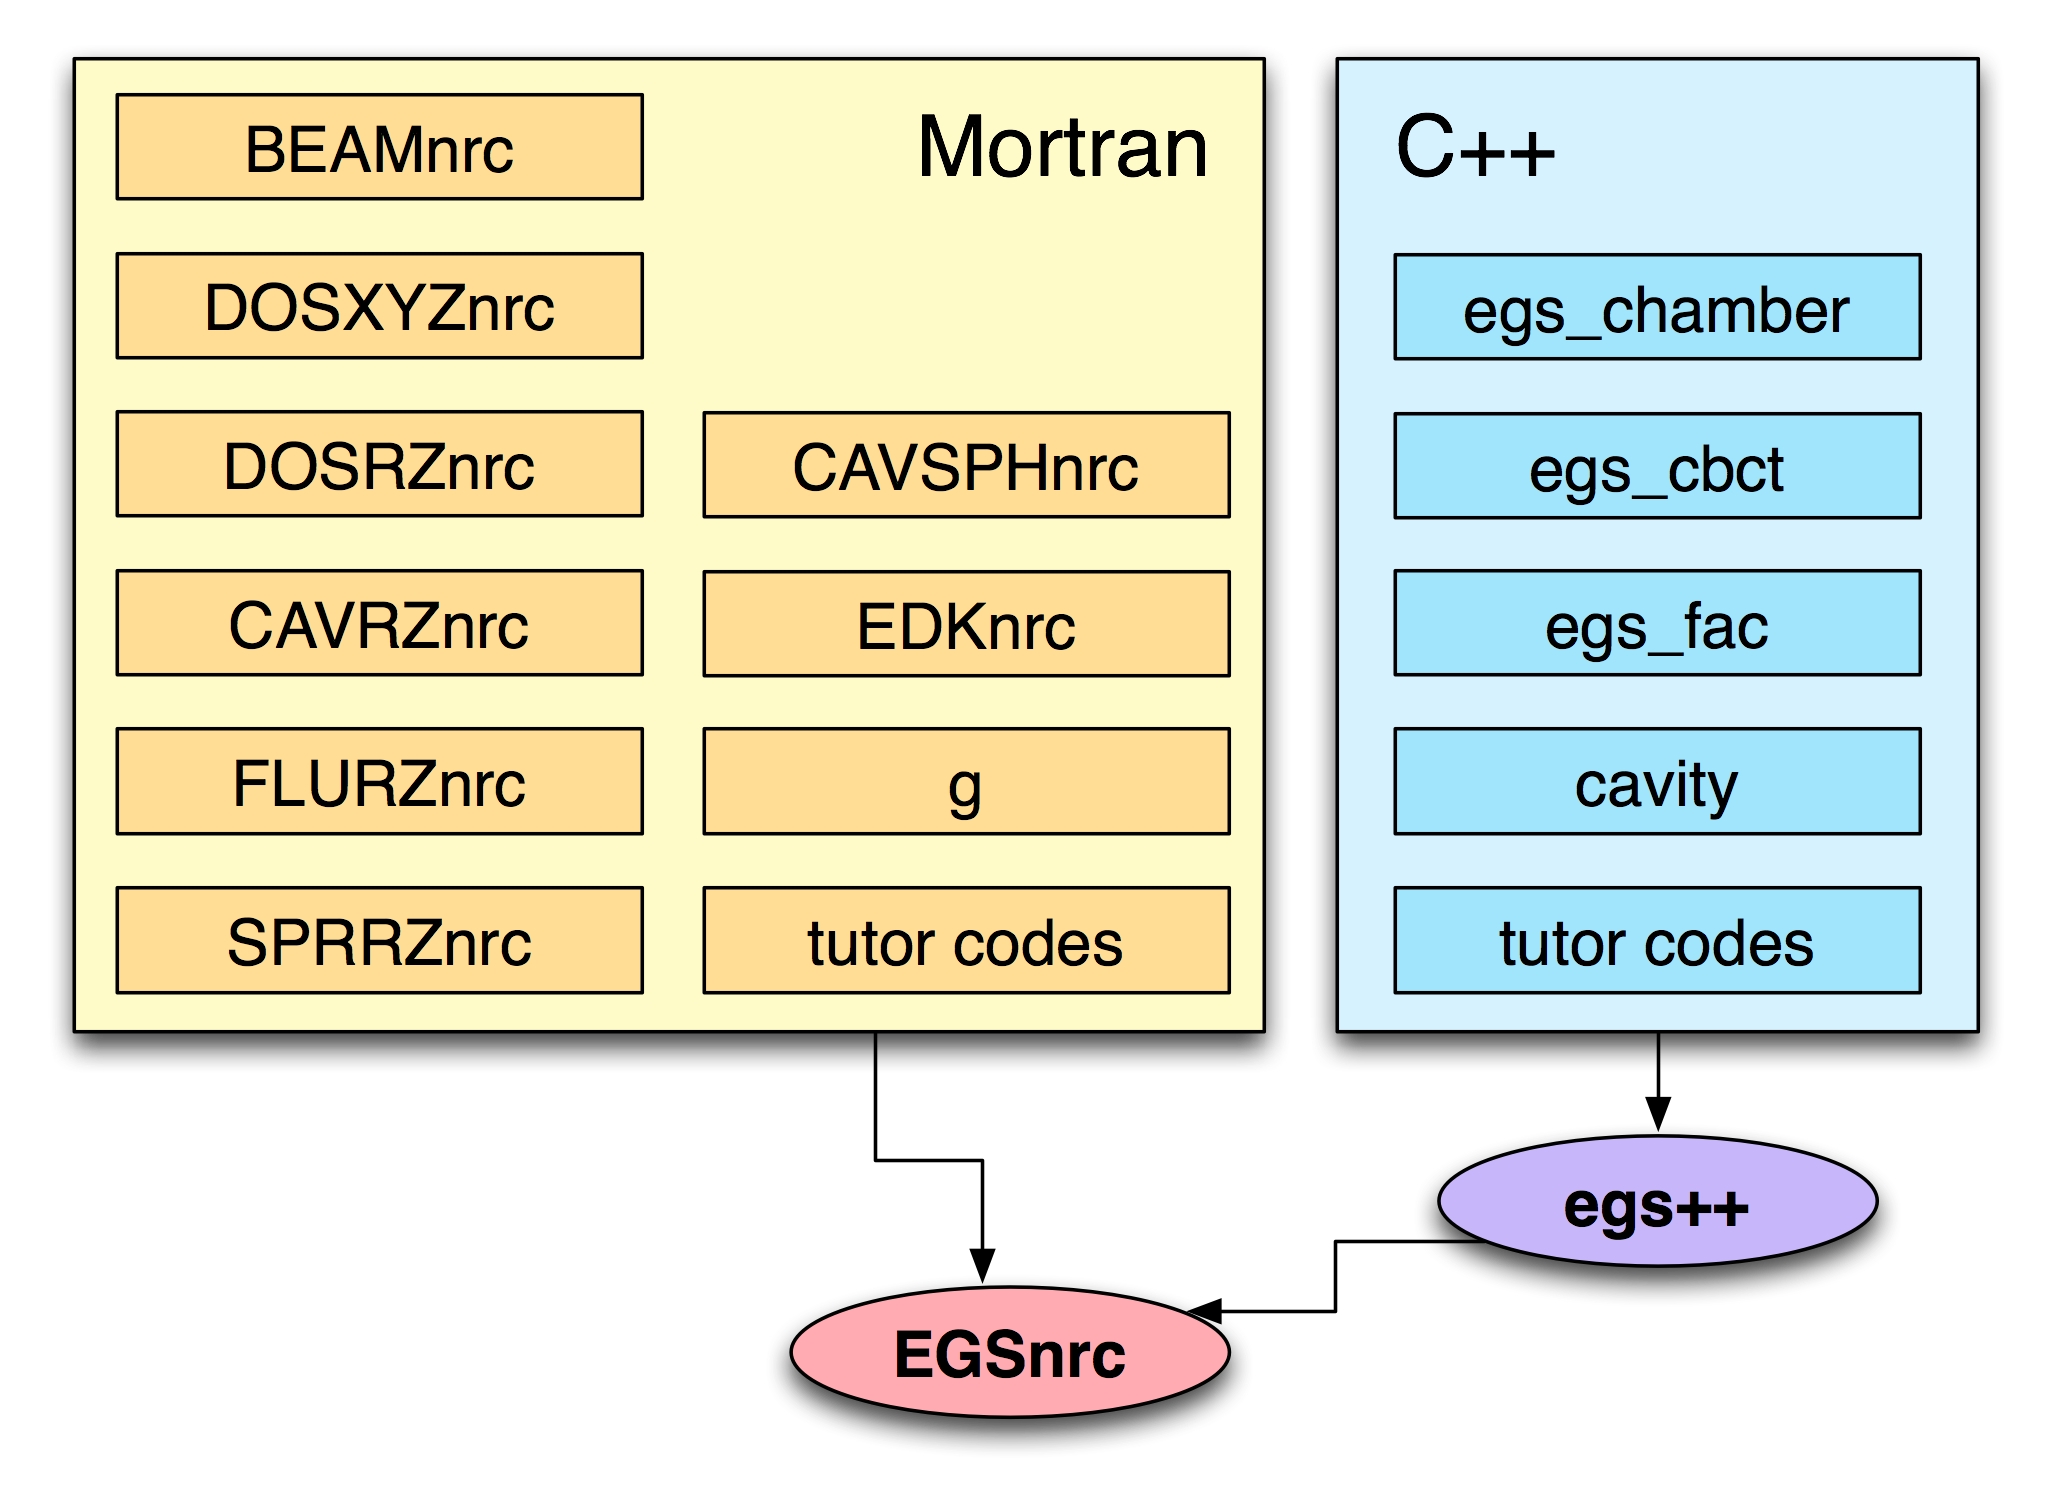
\includegraphics[height=340pt]{figures/egsApplications}
\end{center}

EGSnrc source code: \Verb+$HEN_HOUSE/src/egsnrc.mortran+

EGSnrc global variables: \Verb+$HEN_HOUSE/src/egsnrc.macros+

GUI: \Verb+~/EGSnrc/HEN_HOUSE/gui/egs_gui+

\subsection{BEAMnrc}
\begin{itemize}
\item Ideal for linear accelerator modelling and x-ray systems
\item Includes geometries (called component modules) that can easily represent flattening filters, collimators, MLCs, etc.
\item Accelerators can be compiled as shared libraries to be used as a particle source for other applications
\item Includes time-synchronized capabilities (e.g. dynamic jaws and MLCs)
\item Written in MORTRAN3
\end{itemize}

Documentation: \href{http://nrc-cnrc.github.io/EGSnrc/doc/pirs509a-beamnrc.pdf}{PIRS-509a}

Source code: \Verb+$HEN_HOUSE/omega/beamnrc+

Global variables: \Verb+$HEN_HOUSE/omega/beamnrc/beamnrc_user_macros.mortran+

GUI (launch with \Verb+wish+): \Verb+$HEN_HOUSE/omega/progs/gui/beamnrc/beamnrc_gui.tcl+

\subsection{DOSXYZnrc}
\begin{itemize}
\item Performs dose calculations in voxelized phantoms
\item Includes a variety of source models (e.g. a BEAMnrc shared library)
\item Includes time-synchronized capabilities
\item Written in MORTRAN3
\end{itemize}

Documentation: \href{http://nrc-cnrc.github.io/EGSnrc/doc/pirs794-dosxyznrc.pdf}{PIRS-794}

Source code: \Verb+$HEN_HOUSE/user_codes/dosxyznrc+

Global variables: \Verb+$HEN_HOUSE/user_codes/dosxyznrc/dosxyznrc_user_macros.mortran+

GUI (launch with \Verb+wish+): \Verb+$HEN_HOUSE/omega/progs/gui/dosxyznrc/dosxyznrc_gui.tcl+

\clearpage
\subsection{The RZ applications (cylindrical symmetry)}
These applications are based on cylindrically symmetric geometries and are
written in \Verb+MORTRAN3+. There is a dedicated GUI to compile these
applications and write / edit input files.

Documentation: \href{http://nrc-cnrc.github.io/EGSnrc/doc/pirs702-egsnrc-codes.pdf}{PIRS-702}

GUI documentation: \href{http://nrc-cnrc.github.io/EGSnrc/doc/pirs801-egsinprz.pdf}{PIRS-801}

Source code: \Verb+$HEN_HOUSE/user_codes+

GUI: \Verb+$HEN_HOUSE/gui/egs_inprz+

\subsubsection{DOSRZnrc}
\begin{itemize}
\item Dose and kerma calculations
\end{itemize}
\subsubsection{CAVRZnrc}
\begin{itemize}
\item Calculates ionization chamber correction factors and relevant quantities
\end{itemize}
\subsubsection{FLURZnrc}
\begin{itemize}
\item Particle fluence calculations
\end{itemize}
\subsubsection{SPRRZnrc}
\begin{itemize}
\item Calculates Spencer-Attix spectrum averaged stopping-power ratios for arbitrary media
\end{itemize}

\clearpage
\subsection{The SPH applications (spherical symmetry)}
These applications are based on spherically symmetric geometries and are
written in the fortran preprocessor language \,\Verb|MORTRAN3|.

Documentation: \href{http://nrc-cnrc.github.io/EGSnrc/doc/pirs702-egsnrc-codes.pdf}{PIRS-702}

Source code: \Verb+$HEN_HOUSE/user_codes+

\subsubsection{CAVSPHnrc}
\begin{itemize}
\item Identical to CAVRZnrc but for spherical geometries
\end{itemize}
\subsubsection{EDKnrc}
\begin{itemize}
\item Calculates energy deposition kernels for photons or electrons forced to interact
at the centre of a spherical phantom
\item Also calculates dose distributions in the entire phantom or the dose to specific regions defined as the cavity of a spherical ion chamber
\end{itemize}

\clearpage
\subsection{g}
\begin{itemize}
\item Calculates the energy fraction lost to radiation when electrons slow down (if the incident beam is photons), or the radiative yield (if the incident beam is electrons)
\item Calculates quantities such as mu\_tr, mu\_en and g-bar (the average fraction of energy lost to radiation needed for the calculation of mu\_en)
\item Written in \Verb+MORTRAN3+
\end{itemize}

Source code: \Verb+$HEN_HOUSE/user_codes/g+

\subsection{egs\_chamber}
\begin{itemize}
\item Calculates dose and energy deposited in regions/media
\item Optimized for ionization chamber calculations
\item Many relevant variance reduction techniques
\item Written in c++ (egs++ application)
\end{itemize}

Documentation: \href{http://nrc-cnrc.github.io/EGSnrc/doc/pirs898/egs\_chamber.html}{PIRS-898/egs\_chamber}

Source code: \Verb+$HEN_HOUSE/user_codes/egs_chamber+

\subsection{egs\_cbct}
\begin{itemize}
\item Main goal is the fast estimation of the scatter contribution to an ideal detector in a cone-beam CT (CBCT) setup by means of sophisticated variance reduction techniques and a smoothing algorithm
\item Can also be used for estimating the total signal to the detector and its individual components: transmitted and scattered
\item Initially designed for the purpose of simulating a CBCT setup, but can be equally used for modelling conventional CT scanner setups
\item Written in c++ (egs++ application)
\end{itemize}

Documentation: \href{http://nrc-cnrc.github.io/EGSnrc/doc/pirs898/egs\_cbct.html}{PIRS-898/egs\_cbct}

Source code: \Verb+$HEN_HOUSE/user_codes/egs_cbct+

\subsection{egs\_fac}
\begin{itemize}
\item Designed for the purpose of calculating free air chamber (FAC) correction factors
\item Written in c++ (egs++ application)
\end{itemize}

Documentation: \href{http://nrc-cnrc.github.io/EGSnrc/doc/pirs898/egs\_fac.html}{PIRS-898/egs\_fac}

Source code: \Verb+$HEN_HOUSE/user_codes/egs_fac+

\subsection{cavity}
\begin{itemize}
\item Calculates dose in ionization chamber and correction factors
\item The predecessor of egs\_chamber and egs\_fac
\item Written in c++ (egs++ application)
\end{itemize}

Documentation: \href{http://nrc-cnrc.github.io/EGSnrc/doc/pirs898/cavity.html}{PIRS-898/cavity}

Source code: \Verb+$HEN_HOUSE/user_codes/cavity+

\subsection{Tutorials (the tutor codes)}
\begin{itemize}
\item Many tutorial applications are distributed, written both in \Verb+MORTRAN3+ and c++
\item The codes are heavily documented and intended to teach the user how to write EGSnrc applications
\end{itemize}

Source code: \Verb+$HEN_HOUSE/user_codes+


\clearpage
\section{Getting dirty: writing your first EGSnrc application}
\label{myapp}

Before approaching the more formal descriptions, let's dive right in to actually writing a simple application that will utilize the EGSnrc core physics to perform a Monte Carlo simulation. This hands-on approach will hopefully serve as an instructive lesson on what an EGSnrc application really does, how to write input files and perform simulations, and how to decipher the output.

During the installation, two directories were created and assigned to environment variables: \Verb+$HEN_HOUSE+ and \Verb+$EGS_HOME+. To write an application, navigate to \Verb+$EGS_HOME+ using a file browser, or on the terminal.

If you're working on linux but unfamiliar with environment variables, now might be a good time to do some quick research. Familiarize yourself with basic terminal commands, the shell you are using and the shell configuration (e.g. the \Verb+~/.bashrc+ file if you are using the \Verb+bash+ shell).

\subsection{Create a new egs++ application}

Let's create a new egs++ application called \,\Verb|myapp|. All EGSnrc
applications---including the ones you write yourself---must reside in a
folder with the name of the application, within \,\Verb|$EGS_HOME|.
When we say egs++, we are referring to using the c++ class library that was
built to allow for c++ applications to directly interface with
the \,\Verb|MORTRAN3| EGSnrc core.

Start by creating a new directory for your application, \,\Verb|myapp|.
Then copy the following files from the existing application, \,\Verb|tutor7pp|: \,\Verb|array_sizes.h|, \,\Verb|Makefile|.
We will provide the linux commands to do this, using a bash shell
(the first \Verb|$| on the left represents the \textbf{bash} shell command prompt,
so don't type it in):

\begin{lstlisting}
$ cd $EGS_HOME
$ mkdir myapp
$ cd myapp
$ cp ../tutor7pp/array_sizes.h ./
$ cp ../tutor7pp/Makefile ./
\end{lstlisting}

Open the \,\Verb|Makefile| using your text editor of choice, and change
instances of ``tutor7pp'' to ``myapp''. There are only two lines that need
changing; they should now read:

\begin{lstlisting}
USER_CODE = myapp
\end{lstlisting}

and

\begin{lstlisting}
EGSPP_USER_MACROS = myapp.macros
\end{lstlisting}

Create a new file called \,\Verb|myapp.macros|\,, and just save it as an empty
file. This file is just a a placeholder for now - it may be used by
more advanced applications.

Finally, create a new file named \,\Verb|myapp.cpp|\,, and save the following
source code in it:

\begin{lstlisting}[language=c++,backgroundcolor=\color{white}]
#include "egs_advanced_application.h"
APP_MAIN (EGS_AdvancedApplication);
\end{lstlisting}

This is the smallest, fully functional EGSnrc application you can write\,!
You may consider it a bit of a cheat - we are using the defined function macro
\,\Verb|APP_MAIN| to write some code for us.

Compile your application with the \,\Verb|make|\, command, which builds the
executable \,\Verb|myapp|\, and saves it under \,\Verb|$EGS_HOME/bin/|. For a
given application, you only need to run \,\Verb|make|\, once
(unless you modify the source code). Note that on Windows (if you are using
mingw as the compiler) the compilation command will likely be
\,\Verb|mingw32-make|\, instead.
\begin{lstlisting}
$ make
\end{lstlisting}

\subsection{Create an egs++ input file}

Next we need to create an input file to define the conditions of the simulation.
Create a new file named \,\Verb|slab.egsinp|\, in the application directory,
\,\Verb|$EGS_HOME/myapp/|\,. Copy and paste the following contents:

\begin{lstlisting}[language=ruby,backgroundcolor=\color{white}]
################################
#
# Simple slab simulation
#
################################


################################
### RUN CONTROL
################################
:start run control:
    ncase = 1e3 # The number of histories to simulate
:stop run control:


################################
### GEOMETRY
################################
:start geometry definition: # Only 1 geometry definition block allowed

    ### Define a plate of tantalum
    :start geometry: # Many geometry blocks can be defined
        name     = slab # This name can be anything you like
        library  = egs_ndgeometry
        type     = EGS_XYZGeometry
        x-planes = -5, 5            # in cm
        y-planes = -5, 5            # in cm
        z-planes = -10, 0, 0.1, 10  # in cm
        :start media input:
            media = vacuum tantalum # Indexed as 0 1
            set medium = 1 1 # Set region 1 to medium 1 (tantalum)
                             # Other regions default to medium 0 (vacuum)
        :stop media input:
    :stop geometry:

    ### Use the geometry with this name for the simulation
    simulation geometry = slab

:stop geometry definition:


################################
### MEDIA
################################
:start media definition: # Only 1 media definition block allowed

    # Defining media in the input file like this is called "pegsless" mode

    ### Cutoff energies, in MeV
    ae  = 0.521             # lowest  energy for electrons (kinetic+0.511)
    ap  = 0.01              # lowest  energy for photons   (kinetic)
    ue  = 50.511            # maximum energy for electrons (kinetic+0.511)
    up  = 50                # maximum energy for photons   (kinetic)

    ### Tantalum
    :start tantalum: # this name can be anything
        density correction file = tantalum # name the file (no ext.)
    :stop tantalum:

    ### Lead
    :start lead:
        density correction file = lead
    :stop lead:

    ### Water
    :start water:
        density correction file = water_liquid
    :stop water:

:stop media definition:


################################
### SOURCE
################################
:start source definition: # Only 1 source definition block allowed

    ### Pencil beam
    :start source:
        name      = pencil_beam # This name can be anything you like
        library   = egs_parallel_beam
        charge    = -1
        direction = 0 0 1
        :start spectrum:
            type = monoenergetic
            energy = 20 # in MeV
        :stop spectrum:
        :start shape:
            type     = point
            position = 0 0 -10 # in cm
        :stop shape:
    :stop source:

    ### Use the source by this name for the simulation
    simulation source = pencil_beam

:stop source definition:


################################
### VIEWER CONTROL
################################
:start view control:
    # Here we are just assigning some colors for nice
    # viewing in the egs_view application
    set color = lead      120 120 200 200
    set color = tantalum  120 255 120 255
    set color = water       0 220 255 200
:stop view control:


################################
### AUSGAB OBJECTS
################################
:start ausgab object definition: # Only 1 ausgab definition block allowed

    ### Particle tracks
    :start ausgab object:
        name    = tracks
        library = egs_track_scoring
    :stop ausgab object:

:stop ausgab object definition:
\end{lstlisting}

We'll get into the meaning of the various input parameters later! For now,
let's just run the simulation and see what happens. The input file models
\textbf{a thousand 20~MeV electrons incident on a 1~mm
thick tantalum plate.}

\begin{lstlisting}
$ myapp -i slab.egsinp
\end{lstlisting}

Here \,\Verb|myapp|\, is the executable name, \,\Verb|-i|\, is a
\textit{flag} to specify the input file \,\Verb|slab.egsinp|. This
simulation runs in less than a second and prints results on the
terminal. It also saves information about the simulated particle tracks
in the file \,\Verb|slab.ptracks|.

This command can actually be executed on the terminal from any directory! The myapp executable is found automatically using your \,\Verb|$PATH|\, environment variable, and the input file is \textit{must} reside in the application directory (\,\Verb|$EGS_HOME/myapp|\,)

Load the \,\Verb|slab.egsinp|\, input file and \,\Verb|slab.ptracks|\, in
\,\Verb|egs_view|\, utility to understand the geometry of the simulation.
Click on the scene and drag with the left mouse button to rotate the view.
Zoom in and out with the mouse scroll wheel. Pan
the view by holding Ctrl and dragging with the left mouse button. For more controls, see the \textbf{Controls} section on the \textbf{Camera} tab in the \,\Verb|View Controls| window.

\begin{lstlisting}
$ egs_view slab.egsinp slab.ptracks
\end{lstlisting}

\,\Verb|egs_view|\, should display something
like the following image. In the figure, a pencil beam of electrons is impinging
from the left (negative z), towards the right (positive z).
Notice that by hovering your mouse over the plate, you
can investigate the region numbers that were assigned to the geometry. Looking
down a ray from your mouse, the numbers are displayed in the top left. In this
case, the first region the ray sees is the air above the plate (region 0), then
the Ta plate (region 1), then the air below the plate (region 2). These numbers
that are assigned to geometrical regions are important, as we will see later!

\begin{center}
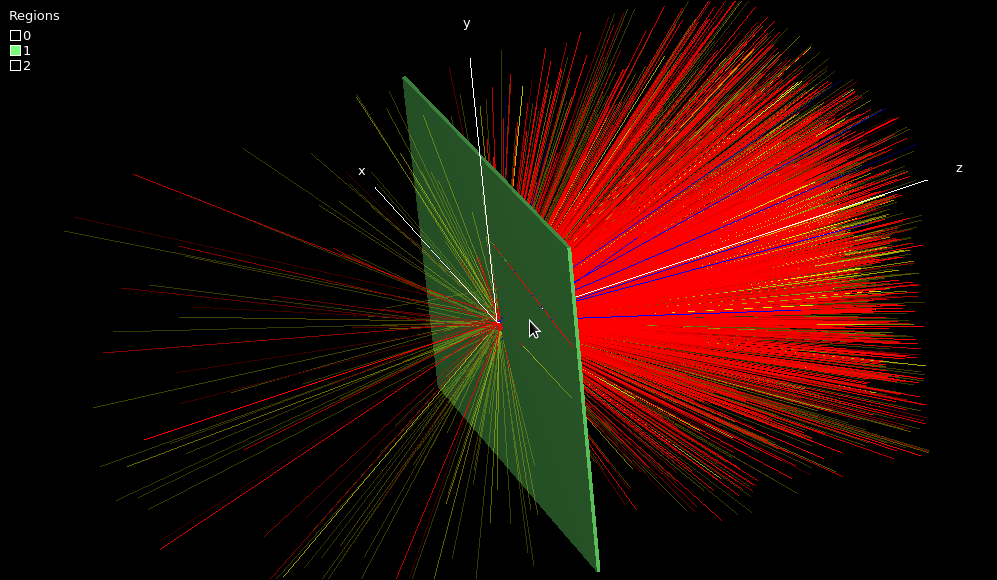
\includegraphics[height=240pt]{figures/ta-plate-example}
\end{center}

Congratulations, you created your first egs++ application and ran
your first simulation\,!

\subsubsection{Questions}

\begin{question}
\item Aside from particle tracks, does the \,\Verb+myapp+\, application
provide any useful information when it runs, such as energy deposited,
dose, spectrum, etc.\,?

\begin{answer}
Not really. By default when an EGSnrc application runs it echoes to the
terminal some information about the simulation configuration,
parameters, data initialization, media definitions, etc. Finally, the
simulation reports progress and some final timing statistics. But in
this first example the result is always zero (and the uncertainty 100\%)
because no physical quantity has been \textit{scored} yet:

{\scriptsize
\begin{lstlisting}[language={},backgroundcolor=\color{white}]
Running 1000 histories

  Batch             CPU time        Result   Uncertainty(%)
==========================================================
      1                0.08              0         100.00
      2                0.16              0         100.00
      3                0.23              0         100.00
      4                0.31              0         100.00
      5                0.40              0         100.00
      6                0.49              0         100.00
      7                0.56              0         100.00
      8                0.64              0         100.00
      9                0.72              0         100.00
     10                0.80              0         100.00


Finished simulation

Total cpu time for this run:            0.80 (sec.) 0.0002(hours)
Histories per hour:                     4.5e+06
Number of random numbers used:          13938479
Number of electron CH steps:            345747
Number of all electron steps:           1.2252e+06
\end{lstlisting}
}
\end{answer}

\end{question}

\clearpage
\subsection{Compile and run using egs\_gui}
All EGSnrc applications can be compiled and run using the GUI, \,\Verb|egs_gui|.
Let's rewind, and repeat the \,\Verb|myapp| example using \,\Verb|egs_gui|
instead of the command line.

\begin{enumerate}
\item Open \,\Verb|egs_gui|\,, the GUI for compiling and executing any EGSnrc application.
\item Notice that the \,\Verb|Compile|\, tab is selected by default. Use the selection box in the bottom left of the GUI, and select \,\Verb|myapp|.
\item Click the \,\Verb|Go|\, button. It will take some time to compile. If you see \,\Verb|ExitCode = 0|\, in the output, the application has compiled successfully! If you are \textit{recompiling} an application, make sure to \,\Verb|clean|\, first.
\item Switch to the \,\Verb|Execute|\, tab.
\item In the \,\Verb|PEGS file|\, section, check the \,\Verb|pegsless|\, checkbox. This means media are defined in the input file.
\item In the \,\Verb|Input file|\, section, click the \,\Verb|...|\, button, and
select the input file we created earlier: \,\Verb|slab.egsinp|.
\item To run the simulation, just click \,\Verb|Start|.
\item The output of the simulation is displayed in the \,\Verb|egs_gui|\, output
textbox after executing the simulation. Depending on the application, there
may be additional output in the corresponding application directory in
\,\Verb|$EGS_HOME|.
\end{enumerate}

\subsection{Add a dose scoring object}

The little application \,\Verb|myapp|\, does not really report any quantity
of interest: by default the egs++ application just transports the
particles in the geometry. It is up to the user to implement methods to
extract information from the simulation.

The easiest way to get results is by adding a dose scoring objects in
your input file. For example, to get a report of the dose deposited in
every region of the geometry at the end of the simulation, \textbf{add}
the following input block \textbf{inside} the existing
\,\Verb|ausgab object definition|\, delimiters at the end of your input
file (you will learn more about the egs++ syntax later). After this, you should
\textbf{only have a single} \,\Verb|ausgab object definition|\,, containing two
\,\Verb|ausgab object|\, blocks.

If your text editor supports syntax highlighting, try setting the language to \textit{ruby}. This does not match our syntax exactly but still helps the eye.

\begin{lstlisting}[language=ruby,backgroundcolor=\color{white}]
:start ausgab object definition:

    # ... there is an existing object here for ptracks

    :start ausgab object:
        name         = dose
        library      = egs_dose_scoring
        dose regions = 1
        volume       = 10
    :stop ausgab object:

:stop ausgab object definition:
\end{lstlisting}

Run the simulation again, and find the ``Summary of region
dosimetry'' in the output:
\begin{lstlisting}
$ myapp -i slab.egsinp
\end{lstlisting}

\subsubsection{Questions}

\begin{question}

\item How much energy is deposited inside the tantalum plate\,? What is
the dose\,?

\begin{answer}
With a dose scoring object, the application echoes additional data to the
screen at the end of the simulation. The energy deposited in the
tantalum plate is ($2.5506\pm1.828$\%)~MeV. The dose is
($2.4535\times10^{-12}\pm1.828$\%)~Gy.

{\scriptsize
\begin{lstlisting}[language={},backgroundcolor=\color{white}]
==> Summary of region dosimetry (per particle)
ir medium      rho/[g/cm3]  V/cm3      Edep/[MeV]              D/[Gy]
-----------------------------------------------------------------------------
1 tantalum  16.654    10.0000 2.5506e+00 +/- 1.828  % 2.4535e-12 +/- 1.828  %
-----------------------------------------------------------------------------
\end{lstlisting}
}
\end{answer}

\clearpage
\item Can you manually convert the value of deposited energy to dose\,?

\begin{answer}
Dose is defined as the energy deposited per unit mass, usually reported
in Gray (J/kg). The density of tantalum here is 16.654~g/cm$^3$, and
the volume of the plate is 10~cm$^3$. Therefore, the mass of the plate
is 166.54~g, and the dose is:
\begin{equation*}
D = \frac{2.5506}{166.54} = 0.015315 \text{\ MeV/g} = 2.4538
\times 10^{-12} \text{\ J/kg}.
\end{equation*}

\end{answer}

\item What is the relative uncertainty on energy and dose, and why is
it the same for both\,?

\begin{answer}
The relative uncertainty on the deposited energy \textit{and} the dose
is 1.828\%. It is exactly the same in both cases because dose is
simply the energy divided the mass. The mass is derived from simulation
inputs which are considered \textit{exact} (the density and the volume),
hence it does not contribute to the relative uncertainty.
\end{answer}

\item Figure out how to increase the number of electrons by a factor 10
in the input file and run the simulation again. Why has the deposited
energy not increased by a factor 10\,? What happened to the uncertainty\,?

\begin{answer}
Changing the run control input to \,\Verb|ncase = 1e4|\, simulates 10$^4$
incident electrons. The deposited energy is now
($2.5893\pm0.572$\%)~MeV. It has not increased by a factor 10 because
Monte Carlo results are reported \textit{per incident particle}. The
relative uncertainty has however decreased by a
factor of about 3, which is typical of a random sampling process, for
which the uncertainty scales like $1/\sqrt{N}$.
\end{answer}

\end{question}


\subsection{Change the type of incident particles}

Figure out how to change the incident particle type to \textit{photons}
instead of electrons in \,\Verb|slab.egsinp|. Save and run the simulation
again for $10^4$ incident photons. Load the particle tracks in
\,\Verb|egs_view|.

\subsubsection{Questions}

\begin{question}

\item Is the simulation faster with electrons or with photons\,?

\begin{answer}
Changing the charge of the source (\Verb|charge = 0|) runs the
simulation for incident photons instead of electrons. The simulation is
about 10 times faster with photons because photons interact with matter
much less than do electrons.
\end{answer}

\item How did the dose change compared to electrons\,?

\begin{answer}
The dose decreased by a factor of about 10 compared to electrons, again
indicating that photons interact less than do electrons.
Correspondingly, the uncertainty is larger than with electrons, because
fewer events are sampled inside the plate.
\end{answer}

\item Are positrons generated in this simulation\,? Is this expected\,?

\begin{answer}
Yes, positrons are generated: they show up as blue tracks in the
viewer. This is expected because the incident photons have an energy
of 20~MeV, well above the pair production threshold of 1.022~MeV.
\end{answer}

\end{question}



\subsection{Change the energy of incident particles}

Figure out how to change the incident particle energy to 1~MeV in
\,\Verb|slab.egsinp|. Save and run the simulation again for $10^4$
incident photons. Load the particle tracks in \,\Verb|egs_view|.

\subsubsection{Questions}

\begin{question}

\item What is the biggest qualitative difference with the 20~MeV
scenario\,?

\begin{answer}
The most striking difference is that there are much fewer
secondary charge particles. Note also that there are no positrons since the incident
energy is now below the pair production threshold of 1.022~MeV.
\end{answer}

\item Did the dose increase or decrease\,?

\begin{answer}
The dose is further decreased to ($5.5088\times 10^{-14} \pm
3.613$\%)~MeV per incident photon.
\end{answer}

\item How about simulation time\,?

\begin{answer}
The simulation time is reduced. As a general rule, lower energy simulations
run faster because there are fewer secondary particles to transport.
\end{answer}

\end{question}



\subsection{Change the material of the plate}

Figure out how to change the material of the plate to \,\Verb|lead|\, in
\,\Verb|slab.egsinp|. Use \textbf{100~keV electrons} and run the
simulation again for $10^4$ incident electrons. Load the particle tracks
in \,\Verb|egs_view|. \textit{Hint:} the materials are set in the
\,\Verb|geometry definition|. The \,\Verb|media definition| defines the list of
media that may (or may not) be used by geometries.

\subsubsection{Questions}

\begin{question}

\item What is happening to the electrons hitting the lead plate\,?

\begin{answer}
The electrons are either absorbed in the lead or backscattered
in the $\,\,-z$ direction.
\end{answer}

\item Is that consistent with the deposited energy\,?

\begin{answer}
Yes, indeed. The energy deposited in the lead plate by 100~keV electrons
is found to be ($0.058803 \pm 0.709$\%)~MeV per incident electron. So on
average only 60\% of the incident energy is deposited in the lead plate,
owing to the significant backscatter.
\end{answer}

\item What is the file size of \,\Verb|slab.ptracks|\, on disk\,?

\begin{answer}
About 5.3~MB. Track files grow very quickly, but by default the number
of events saved to file is limited to 1024, even if you run more
incident particles.
\end{answer}

\item Run 20~MeV electrons striking a \Verb|water| plate
and interpret the results. Is deposited energy consistent with the known
stopping power value of \\
\,\,2.45~MeV~cm$\mathbf{^2}$\!/g\,\, for 20~MeV
electrons in liquid water\,?

\begin{answer}
Most electrons go through the water plate, depositing on average
175~keV in the process. This is certainly \textit{less} than the
energy loss of 245~keV expected from the nominal electron stopping
power, because a lot of energy is carried away from the plate by
secondary particles, mostly bremsstrahlung photons.
\end{answer}

\end{question}

\clearpage
\section{Navigating egs++ input files}
EGSnrc now includes egs++, a C++ class library that interfaces with the EGSnrc core \Verb+MORTRAN3+ code. This allows for applications to be written in C++. To expand on what was covered in the previous section, we will play with one of the egs++ tutorial applications, \Verb+tutor7pp+, and experiment with making changes to the input file.

There is an example input file included with \Verb+tutor7pp+, \Verb+test1.egsinp+, found in the application directory (\Verb+$EGS_HOME/tutor7pp+). Let's run \Verb+tutor7pp+ with this example. If you look inside the \Verb+test1.egsinp+ file, the geometry is defined as an infinite slab of tantalum, 1~mm thick. A parallel beam of 20~MeV electrons is directed at the slab, and the simulation runs 1000000 particles. Additionally, \Verb+tutor7pp+ has special scoring options that are not available to other applications. Each application may define its own input parameters, but generally nearly all of the inputs (e.g. geometries, sources) are the same. For \Verb+tutor7pp+, the application requires some additional inputs that define regions in which to score pulse height distributions (this is at the bottom of the example input file).

Compile and run \Verb+tutor7pp+ using \Verb+egs_gui+, or on the command line.

If you choose to use the command line, the following commands are an example for linux operating systems:
\begin{lstlisting}
$ cd $EGS_HOME/tutor7pp
$ make clean
$ make
$ tutor7pp -i test1 -p tutor_data | tee test1.output
\end{lstlisting}

Notice that we have modified the execution line above to pipe the output to \Verb+tee+ in order to both display it in the terminal as well as save it in an output file. If you look in the application directory after the simulation, it will contain some new files! Namely:
\begin{lstlisting}[backgroundcolor=\color{white}]
test1.egsdat
test1.output
\end{lstlisting}

The \Verb+.egsdat+ file can generally be ignored - it is used by EGSnrc to resume jobs that crashed, or combine parallel runs. The \Verb+.output+ file is where we manually redirected the output from the simulation (if you ran the simulation using the GUI, this file was not created). Looking at the output, we can observe the reflected, deposited and transmitted energy fractions for the simulation of electrons through a single slab. Below this, is the pulse height distribution for region 1 (the slab itself).

\subsection{Write a new input file}
When writing an egs++ input file, you will find yourself frequently referencing the full online documentation, \Verb+PIRS-898+:

\href{http://nrc-cnrc.github.io/EGSnrc/doc/pirs898/index.html}{http://nrc-cnrc.github.io/EGSnrc/doc/pirs898/index.html}

If you would prefer to have a local copy, download all of the manuals (\Verb+EGSnrc-manuals.zip+) from the release page:

\href{https://github.com/nrc-cnrc/EGSnrc/releases}{https://github.com/nrc-cnrc/EGSnrc/releases}

All egs++ applications share the same common input format, though each application may add new input blocks or new input parameters. It is strongly recommended to browse the \Verb+PIRS-898+ documentation on \textit{common inputs}. This will provide an overview of what to expect in an input file:

\href{http://nrc-cnrc.github.io/EGSnrc/doc/pirs898/common.html}{http://nrc-cnrc.github.io/EGSnrc/doc/pirs898/common.html}

To get started writing your first input file from scratch:
\begin{itemize}
\item Open your favourite text editor! \textit{On linux, some editor suggestions are kate, gedit, vim, emacs, etc. On Windows, perhaps notepad++.}
\item There is not a standard syntax highlighter for \Verb+.egsinp+ files. However, you may want to try highlighting for the \Verb+Ruby+ language - it does not match EGSnrc syntax exactly but does do a reasonable job of helping the eye.
\item Save a new file with the \Verb+.egsinp+ extension, in the \Verb+$EGS_HOME/tutor7pp+ directory.
\end{itemize}

To get started with egs++ input files, let's work through an example for the \Verb+tutor7pp+ application. Of course, this example will largely translate to any egs++ application, with the exception of the scoring options, which are specific to \Verb+tutor7pp+. If you read through the \Verb+PIRS-898+ documentation on \href{http://nrc-cnrc.github.io/EGSnrc/doc/pirs898/common.html}{common input blocks}, you will recognize that input files contain:

\begin{itemize}
\item Geometries
\item Particle sources
\item Run control
\item MC transport parameters
\item Media (optional)
\item Ausgab output (optional)
\item Scoring options (application specific)
\end{itemize}

\subsubsection{Define a cylindrical water phantom}

The first step is to define the geometry, which must be placed between the \\
\Verb+geometry definition+ start and stop delimiters in the input file.

First define a cylinder with axis parallel to the $z\!$-axis and 5~cm radius. All distance units in \Verb+.egsinp+ files are in cm, and energy units in MeV.
\vspace{2ex}
\begin{lstlisting}[language=ruby,backgroundcolor=\color{white}]
:start geometry definition:

  :start geometry:
    library  = egs_cylinders
    type     = EGS_ZCylinders
    name     = the_cylinder
    midpoint = 0 0 0 # in cm
    radii    = 5 # in cm
  :stop geometry:

:stop geometry definition:
\end{lstlisting}
\vspace{1ex}

How did we figure out what to type? By looking at the documentation for \href{http://nrc-cnrc.github.io/EGSnrc/doc/pirs898/classEGS__CylindersT.html}{egs\_cylinders}, of course.

The above input block defines an \textit{infinitely long} cylinder of 5~cm radius. To
produce a finite cylinder of 10~cm height with its front face at $z=0$, first
define bounding planes and then put everything together using an ND geometry.
Add these geometries to the geometry definition block:
\vspace{3ex}
\begin{lstlisting}[language=ruby,backgroundcolor=\color{white}]
:start geometry:
    library    = egs_planes
    type       = EGS_Zplanes
    name       = the_planes
    positions  = 0 10 # in cm
:stop geometry:

:start geometry:
    library    = egs_ndgeometry
    name       = phantom
    dimensions = the_planes the_cylinder
    :start media input:
        media = H2O521ICRU
    :stop media input:
:stop geometry:
\end{lstlisting}
\vspace{1ex}

This is one way of creating a \textit{composite geometry}. As described in the \href{http://nrc-cnrc.github.io/EGSnrc/doc/pirs898/classEGS__NDGeometry.html}{egs\_ndgeometry} documentation, the egs\_ndgeometry creates regions where the listed geometries (\Verb+dimensions+) intersect. Since \Verb+the_planes+ contains only one region between $z=0$ and $z=10$, the intersection with \Verb+the_cylinder+ contains a cylinder that has been cut by those planes.

Instead of defining media in the input file, we will be doing it \textit{the old way}. The media used above was \Verb+H2O521ICRU+, which corresponds to the name of a water material defined in an external PEGS data file (\Verb+HEN_HOUSE/pegs4/data/521icru.pegs4dat+). In order to run the simulation (we'll get to this later), the 521icru PEGS4 data file will need to be included as an argument.

Don't forget to tell the \Verb+EGS_Application+ which geometry is the simulation
geometry:
\vspace{1ex}

\begin{lstlisting}[language=ruby,backgroundcolor=\color{white}]
simulation geometry = phantom
\end{lstlisting}

After placing all these blocks into the geometry definition block,
visualize the geometry with \Verb+egs_view+ and enjoy the fruit of your hard
work (of course, use the filename of the input file you just created):

\begin{lstlisting}
$ egs_view yourFile.egsinp
\end{lstlisting}

There is some description of how to use \Verb+egs_view+ in the \href{http://nrc-cnrc.github.io/EGSnrc/doc/pirs898/group__Geometry.html#geometry_view}{geometry module}.

\subsubsection{Define an isotropic point source}

The next step to define the source. Similar to the geometry definition block,
you can define as many sources as desired, create composites, and choose the one to use for
your simulation.

Define an \href{http://nrc-cnrc.github.io/EGSnrc/doc/pirs898/classEGS__IsotropicSource.html}{isotropic point source} of 100~keV photons. This source emits particles uniformly in all directions. Position the source at $-100$~cm from the origin on the $z\!$-axis:
\vspace{2ex}

\begin{lstlisting}[language=ruby,backgroundcolor=\color{white}]
:start source definition:

   :start source:
      library  = egs_point_source
      name     = the_point_source
      position = 0, 0, -100 # in cm
      :start spectrum:
          type   = monoenergetic
          energy = 0.1 # in MeV
      :stop spectrum:
      charge = 0
   :stop source:

   simulation source = the_point_source

:stop source definition:
\end{lstlisting}
\vspace{2ex}

\subsubsection{Define a dose scoring object}

Score dose using the ausgab object \href{http://nrc-cnrc.github.io/EGSnrc/doc/pirs898/classEGS__DoseScoring.html}{egs\_dose\_scoring} which must be defined between the \Verb+:start ausgab object definitions:+ delimiter and corresponding \Verb+stop+ delimiter:
\vspace{2ex}

\begin{lstlisting}[language=ruby,backgroundcolor=\color{white}]
:start ausgab object definition:

    :start ausgab object:
        library     = egs_dose_scoring
        volume      = 785.398163397       # in cm^3
        region dose = yes
        name        = my_dose_scoring
    :stop ausgab object:

:stop ausgab object definition:
\end{lstlisting}

The volume is provided for the cylindrical phantom to be able to compute
the dose. By default volumes are set to 1~cm$\!^3$, so if you do not define the volume, the dose will be incorrect! However, the energy deposited will still be correct, so it is easy to convert to dose after the simulation is complete.

\subsubsection{Define the run control}

The last piece of input required for the simulation to run, albeit with many
defaults, is the number of histories to run, \Verb+ncase+. This value is defined in the \Verb+run control+ block

\begin{lstlisting}[language=ruby,backgroundcolor=\color{white}]
:start run control:
    ncase = 100000
:stop run control:
\end{lstlisting}


\subsection{Run the simulation}

To run the simulation type in the following command. The material data is included using the \Verb+-p+ flag, followed by the name of the PEGS4 data file.

\begin{lstlisting}
$ tutor7pp -i myinput -p 521icru
\end{lstlisting}

Since the output goes to the screen by default, you can \textit{pipe} the output to the \Verb+tee+ command to \textit{simultaneously} save the terminal output to a file, for later analysis of the results:
\begin{lstlisting}
$ tutor7pp -i myinput -p 521icru | tee myoutput.txt
\end{lstlisting}

\subsubsection{Questions}

\begin{question}

\item Compare the energy deposited reported
by the \Verb+egs_dose_scoring+ object and the one corresponding to the fraction
of energy deposited reported by \Verb+tutor7pp+. Are they the same\,?

\begin{answer}
\Verb+tutor7pp+ reports the total energy entering the geometry,
$E_\mathrm{tot}$, and the fractions, $f_i$, of that energy deposited in the
different regions $i$ of the geometry. In this case there is only one region.
The energy deposited in that region, $E_\mathrm{dep}$, is obtained as
\begin{equation*}
 E_\mathrm{dep} = E_\mathrm{tot} \cdot f_0 = 10^4\; \mathrm{MeV} \cdot
0.1934056 = 1934.056\; \mathrm{MeV}
\end{equation*}

The \Verb+egs_dose_scoring+ scoring object reports the dose deposited in each
region $i$ divided by the source's normalization which could be the number of
particles emitted or the fluence. The isotropic point source uses the number of
particles emitted as normalization. Hence to obtain the energy deposited in the
geometry, one has to multiply the reported energy deposited per particle
$\left(\frac{E_\mathrm{dep}}{N}\right)$ by the number of particles emited, $N$
(\Verb+last case+):
\begin{equation*}
 E_\mathrm{dep} = \left(\frac{E_\mathrm{dep}}{N}\right) \cdot N = 1.2082 \cdot
10^{-5}\; \mathrm{MeV} \cdot
160072124 = 1933.991\; \mathrm{MeV}
\end{equation*}

Note above that 10$^5$ is the number of particles hitting the geometry\,!

\end{answer}

\item What is the solid angle, $\Omega$, subtended by the isotropic source and
the front face of the geometry\,?

\begin{answer}
The number of particles emited by the isotropic point source in 4$\pi$ is
160072124, while only 10$^5$ of these particles actually hit the front face of
the cylinder. Hence $\Omega$ can be obtained from
\begin{equation*}
 \Omega = \frac{10^5}{160072124}\cdot 4\pi = 0.00785\; \mathrm{radians}
\end{equation*}

\end{answer}

\item Compute the efficiency $\varepsilon$ based on the uncertainty in the
energy deposited calculated with the \Verb+egs_dose_scoring+ object
and take note of it for a later comparison with the collimated source.

\begin{answer}
\begin{equation*}
\varepsilon = \frac{1}{t_\mathrm{CPU}\cdot \sigma^2} = \frac{1}{0.482^2 \cdot
67.67 s} = 0.0636\; s^{-1}
\end{equation*}
\end{answer}

\end{question}

\subsection{Simulate a collimated source}

Run the same calculation using a collimated source. Add the following source
definition input to the source definition block


{\renewcommand\baselinestretch{1}
\begin{lstlisting}[language=ruby,backgroundcolor=\color{white}]
:start source:
    library  = egs_collimated_source
    name     = my_collimated_source
    distance = 100
    :start source shape:
         type     = point
         position = 0 0 -100
    :stop source shape:
    :start target shape:
         library = egs_circle
         radius  = 5
    :stop target shape:
    :start spectrum:
          type   = monoenergetic
          energy = 0.1
    :stop spectrum:
    charge = 0
:stop source:
\end{lstlisting}
}

Set the simulation source to be \Verb+my_collimated_source+. You may want
to make a copy of your input file.

Run the simulation again by issuing the following command (with your choice of names for the input and output files):

\begin{lstlisting}
$ tutor7pp -i myinput -p 521icru | tee myoutput.txt
\end{lstlisting}


\subsubsection{Questions}

\begin{question}
\item Compare the \textit{fraction} of energy deposited with the result
obtained for the isotropic point source.
Are they the same\,? Explain\,!

\begin{answer}
Although the normalization used by both sources is different, the
fraction of energy deposited in the geometry, $f_0$, is the same within
statistics since as a relative quantity, it should be independent of the
normalization.
\begin{equation*}
 f_0^\mathrm{isotropic} = 0.1934 ,\quad f_0^\mathrm{collimated} = 0.1948
\end{equation*}
\end{answer}

\vspace{-2em}
\item Compare the energy deposited reported by the \Verb+egs_dose_scoring+
object with the same result obtained earlier for the isotropic point source.
Are they the same\,? Explain\,!

\begin{answer}
The collimated source uses the fluence $F$ as normalization. For this reason, the
values reported by the \Verb+egs_dose_scoring+ in this case will be numerically
different from the value reported for the isotropic source:
\begin{equation*}
\frac{E_\mathrm{dep}}{F} = 1.5272\;\mathrm{MeV\; cm^2\;rad.}
\end{equation*}
To get the absolute energy deposited in the geometry, $E_\mathrm{dep}$, one
must use the following expression
\begin{equation*}
E_\mathrm{dep} = \frac{E_\mathrm{dep}}{F} \cdot \frac{N_{\Omega}}{(\Omega
\cdot d\,^2)} = 1.5272 \cdot \frac{10^5}{0.00785 \cdot 10^4} \;\mathrm{MeV}
= 1945.478 \;\mathrm{MeV}
\end{equation*}
This value differs by 0.6 \% from the value obtained for the isotropic
point source which is within the combined uncertainties of the calculations.

\textbf{A side note :} the value reported in this case for the total
energy, called here $E_\mathrm{tot}'$, does not correspond to the actual total
energy $E_\mathrm{tot}$. The quantity $E_\mathrm{tot}'$ is calculated in
\Verb+tutor7pp+ as
\begin{equation*}
E_\mathrm{tot}' = \sum\limits_{i=1}^{N_{\Omega}}{w_i'\, e_i}
\end{equation*}
which for the collimated source actually corresponds to
\begin{equation*}
E_\mathrm{tot}' = E_\mathrm{tot}\cdot \Omega \,.
\end{equation*}
Since the purpose of \Verb+tutor7pp+ is to calculate the energy fractions,
normalization is irrelevant. To get the actual total energy
deposited $E_\mathrm{dep}$ from $E_\mathrm{tot}'$, one needs to use the
expression
\begin{equation*}
 E_\mathrm{dep} = \frac{E_\mathrm{tot}' \cdot f_0}{\Omega}
 = \frac{78.3926\;\mathrm{MeV\;rad} \cdot 0.19482}{0.00785\;\mathrm{rad}} =
1945.535\; \mathrm{MeV}
\end{equation*}
This value is in excellent agreement with the value obtained above from the output of
\Verb+egs_dose_scoring+.
\end{answer}

\item Compute the efficiency based on the uncertainty in the energy deposited
calculated with the \Verb+egs_dose_scoring+ object and compare it with the
efficiency of the isotropic source. Do you see any difference\,?

\begin{answer}
\begin{equation*}
\varepsilon = \frac{1}{t_\mathrm{CPU}\cdot \sigma^2} = \frac{1}{0.362^2 \cdot
3.02 s} = 2.5268\; s^{-1}
\end{equation*}
The collimated source is about \textbf{40 times more efficient} than the
isotropic point source\,!
\end{answer}

\item Can you think of a situation where the collimated source should not be used?

\begin{answer}
The collimated source does not emit particles in all directions, which may not be a good model of reality. If an isotropic source was used instead, the particles directed away from your region of interest \textit{may still contribute to it} by scatter or secondary particles. By collimating the source, these contributions are lost! Thus it is essential to consider whether scatter from the geometry surrounding the source is important for the situation you are modelling.
\end{answer}

\end{question}


\subsection{Generate particles tracks}

And now comes the fun part: \textit{particle tracks\,!}

You will be generating particle tracks with the collimated source. To this end,
you must define an \href{http://nrc-cnrc.github.io/EGSnrc/doc/pirs898/classEGS__TrackScoring.html}{egs\_track\_scoring} object between the
\Verb+ausgab object definition+ delimiters in our input file. Here is an example:
\begin{lstlisting}[language=ruby,backgroundcolor=\color{white}]
:start ausgab object:
    library         = egs_track_scoring
    name            = tracker
    score electrons = no
    score positrons = no
    score photons   = yes
    # start scoring = 0      # default is 0
    # stop  scoring = 1024   # default is 1024
    # buffer size   = 1024   # default is 1024
:stop ausgab object:
\end{lstlisting}

Tracks are only \textit{scored} inside the geometry, hence particle tracks are only generated inside the water cylinder. To see the particle track from the source all the way to the phantom, you need to embed the cylinder and the source inside another geometrical object.

Use a large box of air as an envelope geometry. Add the following two geometries in your geometry definition block:
\begin{lstlisting}[language=ruby,backgroundcolor=\color{white}]
:start geometry:
    library  = egs_box
    box size = 500 500 500
    name     = air_box
    :start media input:
        media = AIR521ICRU
    :stop media input:
:stop geometry:

:start geometry:
   library = egs_genvelope
   name    = phantom_in_air
   base geometry = air_box
   inscribed geometries = phantom
:stop geometry:
\end{lstlisting}

and switch the simulation geometry to be \Verb+phantom_in_air+. Run the
simulation once more with 10 times fewer particles.
This simulation should take a fraction of a second and produce the particle
track file \Verb+myinput.ptracks+. To visualize it launch \Verb+egs_view+ with the name of the tracks file:

\begin{lstlisting}
$ egs_view myinput.egsinp myinput.ptracks
\end{lstlisting}

In the GUI, you can also load the track files afterwards with \Verb+File->Open tracks...+. To get a better view of the tracks and geometry, make the air box transparent (on the \Verb+Colors+ tab) or define a clipping plane. Zoom in for a closer view using the mouse scroll wheel.

\clearpage
\section{Modelling an ionization chamber}
In section \ref{myapp}, we wrote the simplest of egs++ applications and used
\,\Verb|egs_view|\, for the first time. This geometry viewing tool turns out to be
essential when writing complex geometries - both to visually confirm the
accuracy of the design, and to determine the number assigned to \textit{regions}
in the geometry. In the following sections, use this tool frequently!

The \,\Verb|egs_view|\, tool actually uses the \,\Verb|HOWFAR|\,
function of each geometry to render the view. This means that what you see \textit{is
what a particle in your simulation sees}. Note that \,\Verb|egs_view|\, is only
compatible with egs++ input files (not the \,\Verb|MORTRAN3|\, codes).

For more explanation of \,\Verb|egs_view|, refer to the online documentation
for the
\href{http://nrc-cnrc.github.io/EGSnrc/doc/pirs898/group__Geometry.html#geometry_view}{geometry module}.

When trying to simulate a particular experiment, constructing the geometry is
half the battle! Take your time to learn what can be done; starting from
a similar example and tweaking it for your purposes is a key time-saver.
There are geometry examples online, and in the distribution:

\,\Verb|$HEN_HOUSE/egs++/geometry/examples|\,

Before building an ionization chamber, we'll lay a bit more foundation in geometry design and use of \,\Verb|egs_view|. In a text
editor, create a new document with the following geometry input, describing
a cubic box:

{\small
\begin{lstlisting}[language=ruby,backgroundcolor=\color{white}]
:start geometry definition:

    ### a simple box definition
    :start geometry:
        name     = my_box       # this name is up to you
        library  = egs_box
        box size = 10           # length units are cm
        :start media input:
            media = my_medium
        :stop media input:
    :stop geometry:

    ### name of the geometry to load in the viewer
    simulation geometry = my_box

:stop geometry definition:
\end{lstlisting}
}

Note that white space is irrelevant---except for line returns because egs++
reads one input per line. Comment your code as you go, and remember the
\Verb|simulation geometry| input to tell the viewer which geometry to load (by
\textbf{name}).

Media names are up to you: the viewer merely assigns different colors to
different media. These names will ultimately have to be defined in the
\,\Verb|media definition|\, input block (or a PEGS4 data file) to run a simulation.
However, the viewer displays media even if they are not yet defined.

For a description of the egs++ input syntax for each geometry, and for input
examples, refer to the online manual:
\href{http://nrc-cnrc.github.io/EGSnrc/doc/pirs898/index.html}{http://nrc-cnrc.github.io/EGSnrc/doc/pirs898/index.html}, in the
\Verb|Geometries| section, e.g., \Verb|Geometries > EGS_Box|.

\vspace{1ex}
\subsection{Visualize your geometry with {\tt egs\_view}}
\label{sec:box}

Save your box geometry input in a file named \Verb|simple.egsinp|. From the
directory where you saved the file, launch the geometry viewer:

\begin{lstlisting}
$ egs_view simple.egsinp &
\end{lstlisting}

You should see a red square in the geometry window, along with a \textbf{View
Control} window. The viewer starts with the camera on the positive
z-axis, but you can rotate the geometry in 3D by dragging with the mouse, as
shown in figure~\ref{fig:box}a.

You can pan the view by dragging while pressing the \Verb|Ctrl| key, and zoom in
and out with the middle mouse button or the mouse wheel. Note that these
manipulations do \textit{not} affect your input: \Verb|egs_view| \textit{never
writes to the input file.}

Spend a few minutes exploring the tabs to get a feel for what controls are available.
At any time you can
export the current view as an image with \Verb+File->Save image+.

Using \Verb+File->Reload+ the input file will be read again, which is useful to update
the view after making changes. Just keep in mind that if there is a typo in your updated input file, \Verb|egs_view| might crash!

\subsubsection{Question}

\begin{question}

\item What are the region numbers inside and outside the cube\,?

\begin{answer}
When hovering the mouse over the cube, a small red square appears in the top
left corner of the image window, indicating that the inside of the cube is
\textbf{region 0.}

The region \textit{outside} the cube is not displayed in the list. In
egs++ everything outside the defined geometry is \textbf{region\,
$\mathbf{-1}$.} Particles that reach region $-1$ in the simulation are
immediately discarded: they have reached the ``end of the world''\,!
\end{answer}


\end{question}

\vspace{3ex}
\begin{figure}[hb]
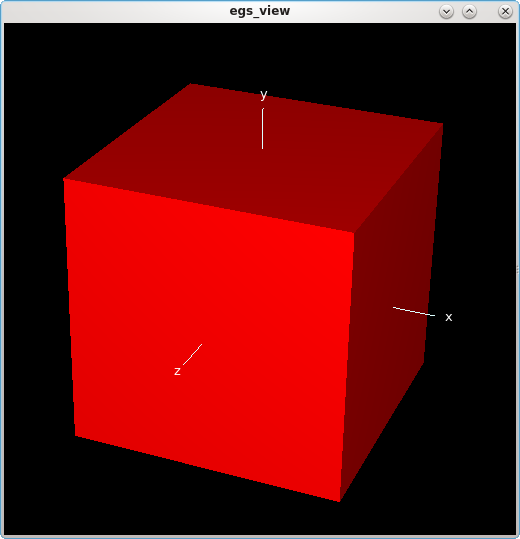
\includegraphics[width=0.49\textwidth]{figures/box}
\hspace{0.02\textwidth}
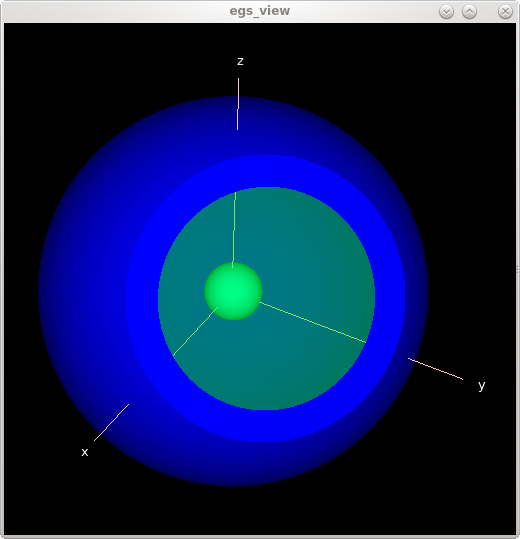
\includegraphics[width=0.49\textwidth]{figures/spheres}
\caption{\label{fig:box} a)~snapshot of the cube defined in the
{\tt simple.egsinp} input file. b)~snapshot of the point of view you
are asked to reproduce using viewer clipping planes in
Section~\ref{sec:clip}.}
\end{figure}


\clearpage
\subsection{\label{sec:clip}Dig in with clipping planes}

Edit your input file to add a second geometry (inside the \textbf{same}
\Verb|geometry definition| input block) defining a set of concentric
spheres:
{\small
\begin{lstlisting}[language=ruby,backgroundcolor=\color{white}]
:start geometry:
    name     = my_spheres   # this name is up to you
    library  = egs_spheres
    radii    = 0.3 1.8 2    # three concentric spheres
    :start media input:
        media = default shell center  # names of media 0 1 2 ...
        set medium = 2 1    # set region 2 to medium 1 (shell)
        set medium = 0 2    # set region 0 to medium 2 (center)
    :stop media input:
:stop geometry:
\end{lstlisting}
}

By default the whole geometry is filled with medium 0 (\Verb|default|, the first
one in the \,\Verb|media|\, list), so it is redundant to specify
\,\Verb|set medium|\, for regions containing medium 0.

Change the \,\Verb|simulation geometry|\, to \,\Verb|my_spheres| (or the name
you
chose) and reload the input in the viewer. You can play with transparency to
reveal the internal structure of the geometry, but clipping planes provide a
more direct route. On the \textbf{Display} tab in \Verb|egs_view|, see the
clipping planes table. Apply a clipping plane oriented along the positive z-axis
and passing through the origin. Make the \Verb|default| medium partially
transparent and rotate the geometry around. Apply a clipping plane to get a view
similar to the one shown in figure~\ref{fig:box}b.

For clipping planes, \Verb|ax|, \Verb|ay| and \Verb|az| define the unit normal
to a planar surface. The surface can then be offset from the origin by setting
the distance \Verb|d| [cm]. After typing in the 4 parameters, hit \textbf{Enter}
to apply the clipping plane, or click away. Use the checkbox to the right of each clipping
plane to toggle them on and off.

\subsubsection{Questions}

\begin{question}

\item From this point of view, what is the list of regions when you hover your
mouse over the small central sphere\,?

\begin{answer}
When hovering the mouse over the central sphere---with a clipping plane as
shown in the figure---the list of regions is \textbf{\{1, 0, 1, 2\}}. These are
all the regions \textit{under} the mouse pointer, from the nearest to the
farthest. Regions clipped by clipping planes are not included in the list.
\end{answer}

\item What is the region number \textit{outside} the defined geometry\,?

\begin{answer}
As always in egs++, the space outside the defined geometry is \textbf{region
$\mathbf{-1}$}, and it is not included in the list of regions in the image
window.
\end{answer}

\end{question}


\subsection{Build an egs++ model of the 3C chamber}

Use your newly acquired expertise in egs++ syntax to model the geometry of NRC's
reference ionization chamber "3C", the schematic of which is reproduced in
figure~\ref{fig:3C}. This is a cylindrically symmetric geometry with 4 distinct
layers along its axis, so the natural option is a \textbf{conestack} geometry.
Put the conestack along the z-axis, and position it according to the numbers
given in the diagram. Below is an input template to get you started. Inspect
the geometry with \Verb|egs_view|.

Read the \href{http://nrc-cnrc.github.io/EGSnrc/doc/pirs898/classEGS__ConeStack.html}{conestack documentation} for more information.

You can expect to end up with 4 layers in the conestack. Since there are no
sloped surfaces (all of the cones are in fact cylinders), the top and bottom
radii will be the same within each layer. Layer 1 requires a single radius,
1.175 for top and bottom. Layer 2 requires two radii for air and graphite,
0.7919 and 1.175, respectively. And so on...

\begin{figure}[ht]
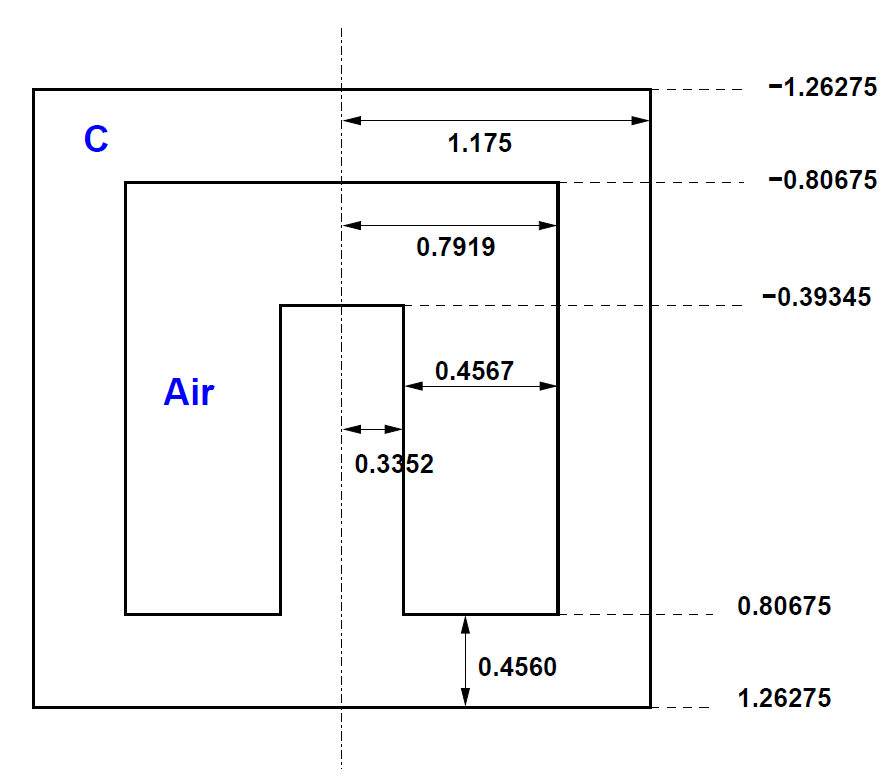
\includegraphics[width=0.7\textwidth]{figures/3C}
\caption{\label{fig:3C} Simplified schematic of NRC's 3C ionization chamber which
is Canada's primary standard for air kerma in a $^{60}$Co beam. Dimensions are in
centimetres. Drawing is not to scale.}
\end{figure}

\vspace{1ex}
{\small
\begin{lstlisting}[language=ruby,backgroundcolor=\color{white}]
:start geometry:
    name    = 3C
    library = egs_cones
    type    = EGS_ConeStack
    axis    = # ... figure out the input for 'axis'

    ### top layer
    :start layer:
        thickness    = # ...
        top radii    = # ...
        bottom radii = # ...
        media        = graphite
    :stop layer:
:stop geometry:
\end{lstlisting}
}

\subsubsection{Questions}


\begin{question}

\item What are the region numbers which correspond to the air cavity\,?

\begin{answer}
The air cavity comprises \textbf{regions 3 and 7.}
\end{answer}

\item Where are regions 1 and 2\,?

\begin{answer}
Regions 1 and 2 are not visible in this geometry: they are \textit{virtual}
regions. In some cases, egs++ attributes region numbers in a way that
is more efficient internally. But the algorithm is deterministic: the same
geometry always yields the same region numbers.
\end{answer}

\item Can you figure out the conestack region numbering scheme\,?

\begin{answer}
In the case of the conestack, egs++ attributes a fixed number of regions to
each layer. This is more efficient because only a single modulo operation is
then needed to convert the region number to the layer index.

In the 3C conestack, there are at most three radii per layer, so egs++
attributes 3 regions per layer, whether or not they are used. The first
layer has only one radial dimension---region 0---hence regions 1 and 2 are not
used: they become \textit{virtual} regions and don't show up in the viewer.
The next layer in the conestack then starts at region 3, and the same logic
applies the virtual region 5.
\end{answer}

\end{question}


\subsection{Build an Exradin A12 chamber}
The Exradin A12 is a thimble ionization chamber, shown schematically in
figure~\ref{fig:a12}. The basic strategy to model such an instrument is to use a
conestack for most of the chamber, which is cylindrically symmetric, except for
the spherical tip. Build the chamber tip with \textbf{spheres} (as shown by
dashed lines in the diagram) and join it with the 7-layer \textbf{conestack}
chamber body, using a composite \textbf{cd geometry}.

\begin{figure}[ht]
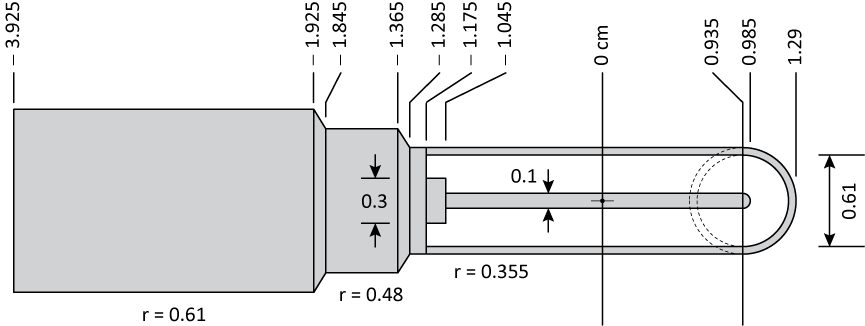
\includegraphics[width=\textwidth]{figures/a12}
\caption{\label{fig:a12}Simplified schematic of an Exradin A12 thimble chamber,
based on information from the manufacturer's product brochure. All units are in
centimetres. Radial dimensions are given, as well as the position of the various
points along the chamber's axis (with the centroid of the collecting volume at
0~cm). The central electrode, the thimble shell and the chamber body are made of
C552 plastic.} \end{figure}

\subsubsection{Model the spherical chamber tip}

Start a new input file for this chamber geometry. Save this input file in
the \\
\,\Verb|$EGS_HOME/egs_chamber| directory. It is recommended to use the
\,\Verb|egs_chamber| application for ionization chamber simulations due to
its useful suite of variance reduction parameters. There are a number of
useful features, found in the \href{http://nrc-cnrc.github.io/EGSnrc/doc/pirs898/egs_chamber.html}{egs\_chamber documentation}.

Define a geometry for the
chamber tip using \textbf{2 concentric spheres,} as in Section~\ref{sec:clip}.
The smallest sphere will become the spherical tip of the central electrode\,!
The outer sphere should be water - the entire chamber will be placed in water
and we will end up using a small water shell surrounding the chamber for a
variance reduction technique called cross section enhancement.
Position the midpoint of the set of spheres on axis in their final location at
$x=0.935$~cm, as shown in figure~\ref{fig:a12}.

{\small
\begin{lstlisting}[language=ruby,backgroundcolor=\color{white}]
#-------------------------------------------------------------------------
# Spherical chamber tip
#-------------------------------------------------------------------------
:start geometry:
    name     = chamber_tip
    library  = egs_spheres
    midpoint = 0.935 0 0
    radii    = 0.05 0.305 0.355 2.0
    :start media input:
        media = c552 air water # media 0,1,2
        set medium = 1 1 # set region 1 to air (1)
        set medium = 3 2 # set region 3 to water (2)
        # by default the rest of the regions are c552
    :stop media input:
:stop geometry:
\end{lstlisting}
}

\textbf{Include the following} bounding
box view control input block in your input file (\textit{outside} the geometry
definition block) to help the viewer find the spheres. Inspect the geometry in
\Verb|egs_view|.

{\small
\begin{lstlisting}[language=ruby,backgroundcolor=\color{white}]
:start view control:
    xmin = -4
    xmax =  4
    ymin = -4
    ymax =  4
    zmin = -4
    zmax =  4
:stop view control:
\end{lstlisting}
}

\subsubsection{Model the chamber body}

Use a \textbf{conestack} to define the cylindrically symmetric chamber body.
Set the axis of the conestack so that layers are added in the -x direction. In
the next step you will join this conestack to the spheres using a cd geometry
plane located at $x=0.935$~cm, so set the top of the conestack at that point.
Surround the chamber in water out to 2~cm radius. See if you can design the
chamber without copy-pasting the text below!

{\small
\begin{lstlisting}[language=ruby,backgroundcolor=\color{white}]
#-------------------------------------------------------------------------
# Main chamber body (as a conestack)
#-------------------------------------------------------------------------
:start geometry:
    name    = chamber_body
    library = egs_cones
    type    = EGS_ConeStack
    axis    = 0.985 0 0 -1 0 0     # x-axis

    ### sensitive volume (cylindrical portion)
    :start layer:
        thickness    = 2.03
        top radii    = 0.05 0.305 0.355 2.0
        bottom radii = 0.05 0.305 0.355 2.0
        media        = c552 air c552 water
    :stop layer:

    ### electrode base
    :start layer:
        thickness    = 0.13
        top radii    = 0.15 0.305 0.355 2.0
        bottom radii = 0.15 0.305 0.355 2.0
        media        = c552 air c552 water
    :stop layer:

    ### up to first kink
    :start layer:
        thickness    = 0.11
        top radii    = 0.355 2.0
        bottom radii = 0.355 2.0
        media        = c552 water
    :stop layer:

    ### first widening
    :start layer:
        thickness    = 0.08
        bottom radii = 0.48 2.0
        media        = c552 water
    :stop layer:

    ### up to second kink
    :start layer:
        thickness    = 0.48
        bottom radii = 0.48 2.0
        media        = c552 water
    :stop layer:

    ### second widening
    :start layer:
        thickness    = 0.08
        bottom radii = 0.61 2.0
        media        = c552 water
    :stop layer:

    ### to end
    :start layer:
        thickness    = 2.0
        bottom radii = 0.61 2.0
        media        = c552 water
    :stop layer:

:stop geometry:
\end{lstlisting}
}

\subsubsection{Join the chamber body to the chamber tip}

Create a set of \textbf{3 planes} perpendicular to the chamber axis, so as to
define two regions, numbered 0 and 1. The middle plane should be located at the
joining point $x=0.935$~cm. The other two planes should be located beyond the
chamber on either side.

{\small
\begin{lstlisting}[language=ruby,backgroundcolor=\color{white}]
### Planes for cd geometry base
:start geometry:
    name      = cd_planes
    library   = egs_planes
    type      = EGS_Xplanes
    # These 3 plane positions define 2 regions for us to use (0 and 1)
    # the outer planes (-4 and 4) could be anything large
    positions = -4 0.935 4
:stop geometry:
\end{lstlisting}
}

Finally, use a \textbf{cd geometry} to combine the chamber body and the chamber
tip, using the planes you just defined as the base geometry. Put the body in
region 0, and the tip spheres in region 1. Verify your geometry visually in
\Verb|egs_view|. The cd geometry package is very useful for combining and
cutting geometries. Check out the
\href{http://nrc-cnrc.github.io/EGSnrc/doc/pirs898/classEGS__CDGeometry.html#details}{relevant documentation}
for more information.

{\small
\begin{lstlisting}[language=ruby,backgroundcolor=\color{white}]
:start geometry:
    name    = chamber
    library = egs_cdgeometry
    base geometry = cd_planes
    set geometry  = 0 chamber_body
    set geometry  = 1 chamber_tip
:stop geometry:
\end{lstlisting}
}

It is important to avoid having surfaces perfectly abutting (touching)
in egs++, so start your cone\-stack at a location $x>0.935$~cm to avoid touching
the conestack surface to the egs\_planes geometry. To do this, make the top layer
slightly thicker (say 0.05~cm thicker, making it
$1.045+.935+.05=2.03$~cm), and position the conestack at
$0.935+0.05=0.985$~cm to effectively bleed the conestack into the other
geometry. The cd geometry will cut this extra bit off at the plane we define,
giving priority to the chamber tip.

\begin{center}
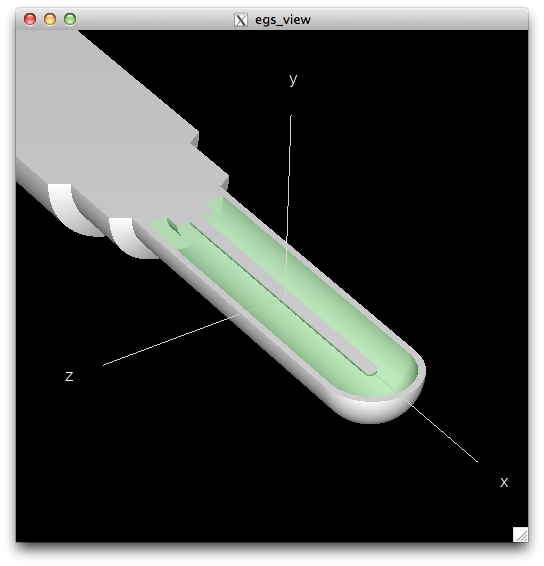
\includegraphics[height=240pt]{figures/a12view}
\end{center}

\subsubsection{Questions}

\begin{question}

\item What are the region numbers that correspond to the air cavity\,?
\textit{Hint: Use a clipping plane (0,1,0,0) in \,\Verb|egs\_view|.}

\begin{answer}
The air cavity is comprised of \textbf{regions 1, 5 and 29.}
\end{answer}

\item Why is the region number for the spherical tip of the air cavity so large\,?

\begin{answer}
The spherical tip of the air cavity is region 29, because the conestack is
added first in the cd geometry. Therefore, region numbers are attributed
first to the conestack (regions 0 to 27, for 7 layers $\times$ 4 regions per
layer), and only then to the spherical regions in the chamber tip.
\end{answer}

\item How many regions are there in total in this model\,? How
many \textit{real} regions\,?

\begin{answer}
There are \textbf{32 regions} in this chamber model, ranging from 0 to 31.
However, there are many \textit{virtual} regions in the chamber stem, where
there are only two radii per conestack layer. There are 10 virtual regions,
hence there are only \textbf{22 real regions} in the geometry.
\end{answer}

\item What is the largest region number in this geometry\,?

\begin{answer}
The largest region number in this geometry is \textbf{31} (the chamber tip
shell). Keep in mind that region numbering starts from 0, so if a geometry
contains $n$ regions, the largest region number is $n-1$.
\end{answer}

\end{question}

\subsubsection{Add a region label for the cavity}
You have already determined the region numbers for the cavity, but what happens
if you add more components to the geometry? The \textit{global} region number might
change! For example, if we inscribe the chamber in a box of water and look
at the region numbers of the cavity again, they will be different. If you need
to know the cavity region numbers for scoring quantities (we will), this can
be quite inconvenient. Instead, use region labels. This assigns a series
of \textit{local} region numbers within a given geometry to a label that you can reference
elsewhere.

Local region numbers are what you find when viewing a particular geometry
(e.g. our geometry by the name of \,\Verb|chamber|). To find the local
region numbers just set that geometry as the calculation geometry, and
open \,\Verb|egs_view|. In contrast, the \textit{global} region numbers are the
numbers that get assigned to those same regions when the geometry gets included
in a more complex \textit{composite} geometry. For example, the composite geometry
of a chamber inscribed in water.

To add a region label, place the following \textit{within a geometry block}.
In this example we give the label the name \,\Verb|chamber_cavity_label|\,
(make sure it's unique!) and assign the local regions 1, 5 and 29
(the air cavity regions). Now if we want to reference those regions elsewhere
in the input file,
we can reference the \textit{label} instead of the global region numbers
(which may change if other geometries in the input file are modified).

{\small
\begin{lstlisting}[language=ruby,backgroundcolor=\color{white}]
set label = chamber_cavity_label 1 5 29
\end{lstlisting}
}

Add region labels both for the air cavity regions, and for the entire chamber.
The latter of these will be used for a variance reduction technique.

{\small
\begin{lstlisting}[language=ruby,backgroundcolor=\color{white}]
### Join tip and body, attached at the cd_planes
:start geometry:
    name    = chamber
    library = egs_cdgeometry
    base geometry = cd_planes
    set geometry  = 0 chamber_body
    set geometry  = 1 chamber_tip

    # The label for the cavity regions
    # View the chamber geometry alone to find these numbers
    set label = chamber_cavity_label 1 5 29
    set label = chamber_xcse 0 1 2 3 4 5 6 7 8 9 10 11 12 13 14 15 16 17 \\
                18 19 20 21 22 23 24 25 26 27 28 29 30 31
:stop geometry:
\end{lstlisting}
}

\subsubsection{Inscribe the chamber in air}

Now that the chamber has the sensitive regions labelled, inscribe it in a box
of water, then in a larger box of air. There are many ways to do this!
Name the new composite geometry
\,\Verb|chamber_in_water_in_air|, and set it to be the new simulation geometry
(there can only be one).

View the geometry in \,\Verb|egs_view|\, again, setting air and water
transparent and using a clipping plane. Notice how the region numbers of the
sensitive volume of the chamber have changed - this is the motivation for
region labels.

{\small
\begin{lstlisting}[language=ruby,backgroundcolor=\color{white}]
#-------------------------------------------------------------------------
# A water and air box surrounding the chamber
#-------------------------------------------------------------------------

# Air outside whole structure
:start geometry:
    name        = outer_air_box
    library     = egs_box
    box size    = 15 15 210
    :start media input:
        media = air
    :stop media input:
:stop geometry:

# Water outside the chamber
:start geometry:
    name        = water_box
    library     = egs_box
    box size    = 10
    :start media input:
        media = water
    :stop media input:
:stop geometry:

# Inscribe the chamber in the water
:start geometry:
    name = chamber_in_water
    library = egs_genvelope
    base geometry = water_box
    inscribed geometries = chamber
:stop geometry:

# Inscribe the water and chamber in the air
:start geometry:
    name = chamber_in_water_in_air
    library = egs_genvelope
    base geometry = outer_air_box
    inscribed geometries = chamber_in_water
:stop geometry:

simulation geometry = chamber_in_water_in_air
\end{lstlisting}
}

\subsubsection{Add media definitions}
Add media definitions to the input file (pegsless mode). Assign the same names
that we used to media in the geometry (air, c552, water), and set the density
correction files appropriately. The full set of density correction files
distributed with EGSnrc
can be found in \,\Verb|$HEN_HOUSE/pegs4/density_corrections/|. If the
density correction file you are using resides in that directory, or in
\,\Verb|$EGS_HOME/pegs4/density_corrections/|, then the `.density` extension
can be omitted. To use a density correction file located elsewhere, type
the full path and file extension.

The big benefit of this style of media definition is the ability to set
\,\Verb|AE|\, and \,\Verb|AP|\, in the input file. Previously it was necessary
to generate a new pegs4 data file each time these parameters were changed
(the 521 in \,\Verb|521icru|\, refers to the \,\Verb|AE|\,).

{\small
\begin{lstlisting}[language=ruby,backgroundcolor=\color{white}]
##############################################################################
### Media definition
##############################################################################
:start media definition:

    ### Cutoff energies
    ae  = 0.521             # lowest  energy for electrons (kinetic+0.511)
    ap  = 0.01              # lowest  energy for photons   (kinetic)
    ue  = 50.511            # maximum energy for electrons (kinetic+0.511)
    up  = 50                # maximum energy for photons   (kinetic)

    # I chose the name 'air', use something easy to type
    :start air:
        # .density extension omitted for density correction files located in
        # $HEN_HOUSE/pegs4/density_corrections or $EGS_HOME/pegs4/density_corrections
        density correction file    = air_dry_nearsealevel
    :stop air:

    :start c552:
        density correction file    = c-552air-equivalentplastic
    :stop c552:

    :start water:
        density correction file    = water_liquid
    :stop water:

:stop media definition:
\end{lstlisting}
}

\subsubsection{Add a particle source}
Add a simple collimated 10~MeV photon source. The source shape should be a point,
positioned at -100~cm on the z-axis. Set the target shape to be a rectangle
at the origin, $10\times10$ cm$^2$.

To model a linear accelerator instead,
you will need to replace this with a \href{http://nrc-cnrc.github.io/EGSnrc/doc/pirs898/classEGS__BeamSource.html}{BEAMnrc shared library source}, or a \href{http://nrc-cnrc.github.io/EGSnrc/doc/pirs898/classEGS__PhspSource.html}{phase-space source}.

{\small
\begin{lstlisting}[language=ruby,backgroundcolor=\color{white}]
##############################################################################
### Source definition
##############################################################################
:start source definition:

    :start source:
        name    = photons
        library = egs_collimated_source
        charge  = 0
        :start source shape:
            type = point
            position = 0 0 -100
        :stop source shape:
        :start target shape:
            library = egs_rectangle
            rectangle = -5 -5 5 5
        :stop target shape:
        :start spectrum:
            type = monoenergetic
            energy = 10
        :stop spectrum:
    :stop source:

    simulation source = photons

:stop source definition:
\end{lstlisting}
}

\subsubsection{Add transport parameters and run control}
For ionization chamber simulation, it is OK to use most of the EGSnrc default
settings. There are two parameters that you should always set manually:
the total energy cut-offs for electrons and photons, \,\Verb|ECUT|\,
and \,\Verb|PCUT|\,, respectively.

Why are these parameters so important? In short, they constitute a stage in the
simulation where approximations may occur. Particles whose total energy fall
below the cut-off are absorbed in the current region, depositing all energy
and no longer being transported. This means that secondary particles will no
longer be produced, so even if the energy of the particle was so low that it
would not leave the current region, there is a loss of secondary production. For
this reason, it is essential to set \,\Verb|ECUT|\, and \,\Verb|PCUT|\,
sufficiently low. However, smaller cut-off values means longer simulation times,
and in some cases result in negligible changes to quantities of interest.

For now, use \,\Verb|ECUT=0.521|\, and \,\Verb|PCUT=0.01|.

{\small
\begin{lstlisting}[language=ruby,backgroundcolor=\color{white}]
:start MC transport parameter:
    Global Ecut                 = 0.521
    Global Pcut                 = 0.01
:stop MC transport parameter:

:start run control:
    ncase = 1e5 # simulate 10^5 source particles
:stop run control:
\end{lstlisting}
}

\subsubsection{Add egs\_chamber scoring options}
The scoring options in this section can be used only in input files for the
\,\Verb|egs_chamber|\, application.

Calculate the cavity mass (in grams) by determining the volume of each air cavity region,
then multiplying by the density of air. To be consistent with the simulation,
use the density that is the 3rd value in the air density correction file.

To use the variance reduction technique photon cross-section enhancement, set
the \\
\,\Verb|enhance regions|\, to all of the chamber regions, and the value of
\,\Verb|enhancement|\, to $-128$. The negative value of \,\Verb|enhancement|\,
sets the same value to all of the regions. This will cause photons to interact
with 128 times higher probability within the chamber, resulting in more
electron production and energy deposition in the cavity region. This is a true
variance reduction technique and does not degrade accuracy in any way.

{\small
\begin{lstlisting}[language=ruby,backgroundcolor=\color{white}]
##############################################################################
### Scoring options
##############################################################################
:start scoring options:
    :start calculation geometry:
        geometry name   = chamber_in_water_in_air # The simulation geometry
        cavity regions  = chamber_cavity_label # Air cavity regions
        cavity mass     = 0.00080152267 # g, used density = 1.20478997E-03 g/cm^3
        cavity geometry = chamber # For russian roulette
        enhance regions = chamber_xcse # All the chamber regions
        enhancement     = -128 # Use negative to set the same for all regions
    :stop calculation geometry:
:stop scoring options:
\end{lstlisting}
}


\subsubsection{Add variance reduction}
Turn on photon cross section enhancement using the variance reduction input
block.  These variance reduction parameters are valid
\textit{only for egs\_chamber}, and are designed specifically for high
efficiency in ionization chamber simulations.

Since a cross-section enhancement of 128 was set in the scoring options, turn
on Russian Roulette using the \,\Verb|rejection|\, input, setting it to 128.
Then 1/128 will be the probability for survival in a Russian Roulette game
played with electrons that cannot reach the cavity.

We will not be using electron range rejection, so set \,\Verb|Esave|\, to
the same value as \,\Verb|ECUT|.

{\small
\begin{lstlisting}[language=ruby,backgroundcolor=\color{white}]
##############################################################################
### Variance reduction
##############################################################################
:start variance reduction:

    # Turn on photon cross-section enhancement (xcse)
    cs enhancement  = 1

    # Turn on Russian Roulette for electrons that cannot reach the cavity
    :start range rejection:
        rejection       = 128 # 1/128 is the Russian Roulette survival probability
        Esave           = 0.521 # The energy below which electrons that are in the
                                # cavity and cannot escape the current region
                                # are immediate discarded and energy deposited
                                # 0.521 (same as ecut) implies no range rejection
        cavity geometry = chamber
        rejection range medium = air # Not using range rejection so this
                                     # doesn't matter
    :stop range rejection:

:stop variance reduction:
\end{lstlisting}
}


\subsubsection{Add ausgab (output) options}
Of course the most useful part of a simulation is the output! This is done
using \,\Verb|ausgab|\, objects. Include one for track scoring and one for
dose scoring.

\textbf{Important note:} currently, track scoring is incorrect when used with variance
reduction techniques turned on. The simulation results are unchanged, but the
tracks paths are incorrect. In order to view tracks and avoid this problem,
comment out the variance reduction input block before running a very short
simulation just for track generation. Comment out the tracks ausgab object
for long simulations.

To list the dose in each of the cavity regions, use the label that was defined
as \\
\,\Verb|chamber_cavity_label|. Then, for the regions in order of increasing
number, calculate and provide the
\,\Verb|volume|\, for each region. This is used to calculate dose from the
energy deposited in each region. If you are only interested in the energy
deposited, you can neglect this input.

In the example below, notice that particle track scoring is commented out.
It is possible to comment out an entire input block by just commenting out the
\,\Verb|:start|\, line.

{\small
\begin{lstlisting}[language=ruby,backgroundcolor=\color{white}]
##############################################################################
### Ausgab
##############################################################################
:start ausgab object definition:
    #:start ausgab object:
        name    = tracks
        library = egs_track_scoring
        stop scoring = 1000
    :stop ausgab object:
    :start ausgab object:
        library      = egs_dose_scoring
        name         = doseScoring
        medium dose  = yes
        # List of individual regions
        dose regions = chamber_cavity_label
        # List of each region volume (in same order), cm^3
        volume = 0.57732 0.02880 0.05916
    :stop ausgab object:
:stop ausgab object definition:
\end{lstlisting}
}


\subsubsection{Run the simulation}
Run the simulation! Make sure that your input file resides in the \,\Verb|$EGS_HOME/egs_chamber|\, directory, and has the \,\Verb|.egsinp|\, extension.
It is only necessary to compile \,\Verb|egs_chamber|\, if you have not done
so previously. On linux systems, run \,\Verb|egs_chamber|\, using the following
command (replacing the input/output file names accordingly). Alternatively,
use \,\Verb|egs_gui|.

\begin{lstlisting}
$ egs_chamber -i yourInput.egsinp | tee yourOutput.txt
\end{lstlisting}

Once the simulation is complete, the output near the end should look something
like the following (the example simulated 10$^6$ histories).

{\scriptsize
\begin{lstlisting}[language={},backgroundcolor=\color{white}]
 last case = 1000000 fluence = 1e+06

Geometry                        Cavity dose
-----------------------------------------------
chamber_in_water_in_air   2.1911e-15 +/- 1.081  %



======================================================
Dose Scoring Object(doseScoring)
======================================================
=> last case = 1000000 fluence = 1e+06


==> Summary of region dosimetry (per particle)
ir medium    rho/[g/cm3]  V/cm3      Edep/[MeV]              D/[Gy]
-------------------------------------------------------------------------------
 3 air     0.001     0.5773 9.4809e-09 +/- 1.125  % 2.1836e-15 +/- 1.125  %
 7 air     0.001     0.0288 4.7904e-10 +/- 2.005  % 2.2117e-15 +/- 2.005  %
31 air     0.001     0.0592 1.0028e-09 +/- 1.921  % 2.2538e-15 +/- 1.921  %
-------------------------------------------------------------------------------


==> Summary of media dosimetry (per particle)
medium        Edep/[MeV]              D/[Gy]
--------------------------------------------------------
c552  6.5399e-05 +/- 3.936  % 9.3737e-16 +/- 3.936  %
air   3.1250e-05 +/- 1.086  % 3.3441e-12 +/- 1.086  %
water 1.1111e-02 +/- 0.477  % 3.4258e-13 +/- 0.477  %
--------------------------------------------------------

======================================================
\end{lstlisting}
}


\subsubsection{Questions}

\begin{question}

\item What is the total dose deposited to the ionization chamber cavity? Why is
this different from the total dose to air?

\begin{answer}
The total dose to the air cavity is NOT the sum of the dose to regions 3, 7 and 31.
Instead, there are two alternative methods. First is the pedagogical approach:
use the energy deposited and the mass (or density multiplied by volume) of the combined regions, as well as the conversion factor for MeV/g to Gy, 1.602e-10.

\begin{equation*}
D = \frac{E_1 + E_2 + E_3}{m_1 + m_2 + m_3}
\end{equation*}
\begin{equation*}
= (\frac{9.4809e-09 + 4.7904e-10 + 1.0028e-09}{0.001*(0.5773 + 0.0288 + 0.0592)})*1.602e-10
\\
= 2.6398e-15
\end{equation*}

The second method is to add the doses weighted by the volume. In theory this should give the same answer, but due to the limited number of significant figures printed in the output,
the result is not the same. For that reason, this is the more accurate method. Note that we have eliminated dependency on density because all the regions are of equal density - it is
left as an exercise to the reader to show the equivalency with the first method.
\begin{equation*}
D = D_1 * \frac{V_1}{V} + D_2 * \frac{V_2}{V} + D_3 * \frac{V_3}{V}
\end{equation*}
\begin{equation*}
= 2.1836e-15*0.5773/0.6653 + 2.2117e-15*0.0288/0.6653 + 2.2538e-15*0.0592/0.6653
\\
= 2.1911e-15
\end{equation*}

The total dose to the cavity is smaller than the total dose to air under
\textit{Summary of media dosimetry}, because the total dose to air includes the
dose to additional air regions outside the chamber.
\end{answer}

\end{question}


\clearpage
\section{Linear accelerator simulations}
The BEAMnrc application has long been the workhorse for linear accelerator (LINAC) simulations using EGSnrc. It has been used by many clinical groups to build radiotherapy modelling systems. In such situations BEAMnrc is typically coupled with a second application to perform voxelized transport (e.g. patient modelling), like DOSXYZnrc, vmc++ or any egs++ application.

BEAMnrc is distributed with a powerful GUI that enables the user to easily create new accelerators, compile them, design input files and run simulations. It requires the tcl/tk packages to be installed, as mentioned in the installation instructions. To launch the GUI, either find the shortcut on your desktop or in a linux terminal type:

\begin{lstlisting}
$ beamnrc_gui
\end{lstlisting}

\subsection{Build a new BEAMnrc accelerator}
In the BEAMnrc GUI, click \,\Verb|File -> Specify a new accelerator| (figure \ref{fig:beamnrc_specifyNew}). In the window that pops up (figure \ref{fig:beamnrc_specifyNew2}), select \,\Verb|SYNCJAWS|\, and click \,\Verb|>>|. Type in any name for the component module under \,\Verb|CM Identifier|\,, and click \,\Verb|Add| then \,\Verb|Save & close|.

\begin{figure}
\begin{center}
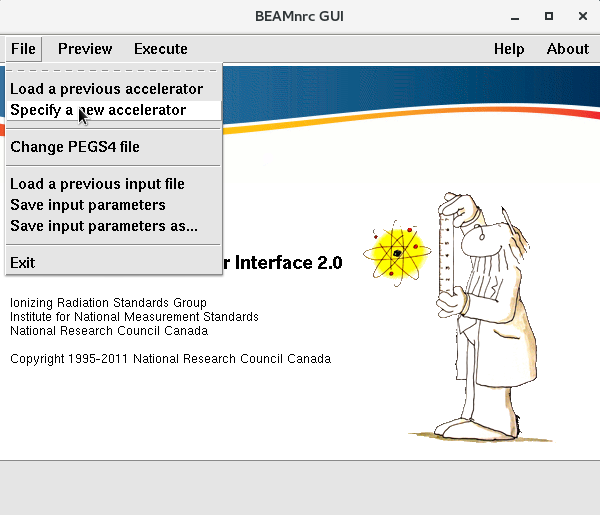
\includegraphics[width=5in]{figures/beamnrc_specifyNew}
\caption{BEAMnrc: Creating a new accelerator}
\label{fig:beamnrc_specifyNew}
\end{center}
\end{figure}

\begin{figure}
\begin{center}
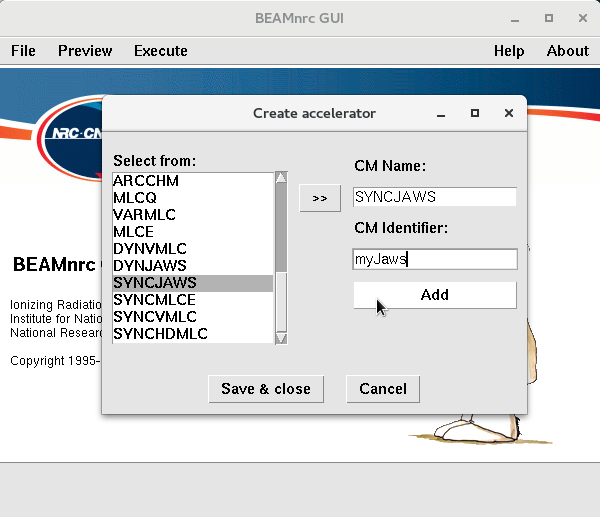
\includegraphics[width=4in]{figures/beamnrc_specifyNew2}
\caption{BEAMnrc: Selecting components}
\label{fig:beamnrc_specifyNew2}
\end{center}
\end{figure}

Save the accelerator module file as \,\Verb|syncjaws.module|\, - this will provide the name of the accelerator. The next window (figure \ref{fig:beamnrc_specifyNew3}) allows you to select the material data to use. Click \,\Verb|Browse HEN_HOUSE|\, and select \,\Verb|700icru.pegs4dat|.

\begin{figure}
\begin{center}
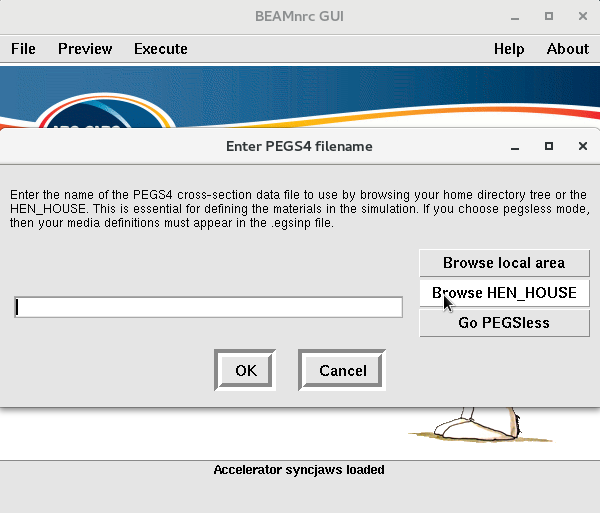
\includegraphics[width=4in]{figures/beamnrc_specifyNew3}
\caption{BEAMnrc: Selecting materials}
\label{fig:beamnrc_specifyNew3}
\end{center}
\end{figure}

Compile the accelerator! In the main BEAMnrc GUI window, go to \,\Verb|Execute -> Compile|\, and click \,\Verb|Build & Compile|\,, as in figure \ref{fig:beamnrc_compile}.

\begin{figure}
\begin{center}
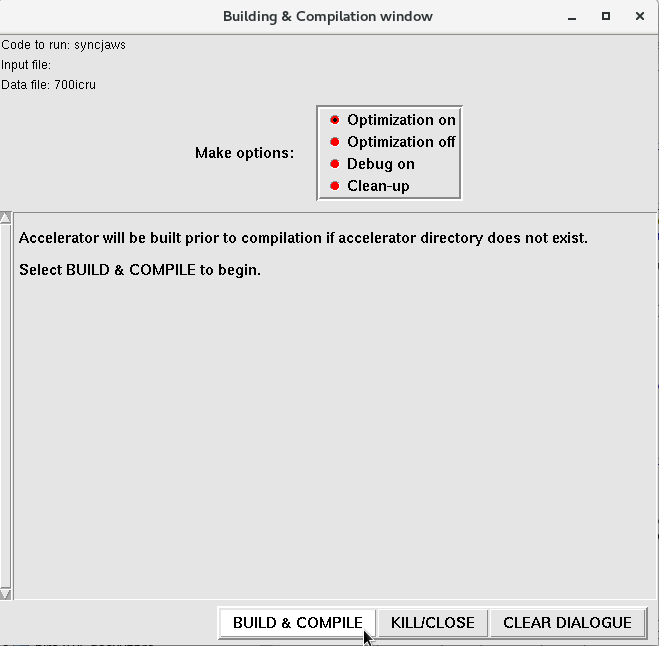
\includegraphics[width=5in]{figures/beamnrc_compile}
\caption{BEAMnrc: Compiling an accelerator}
\label{fig:beamnrc_compile}
\end{center}
\end{figure}

Now you are ready to start editing a new input file. To do this, click on \\
\,\Verb|Edit main input parameters|\, in the \,\Verb|Selected components|\, window. Set a title, and change the parameters to match figure \ref{fig:beamnrc_mainInputs}. When selecting source 1, set the parameters as in figure \ref{fig:beamnrc_source1}. For scoring options, set a plane to be scored after the jaws (component 1) as in figure \ref{fig:beamnrc_scoring}.

\begin{figure}
\begin{center}
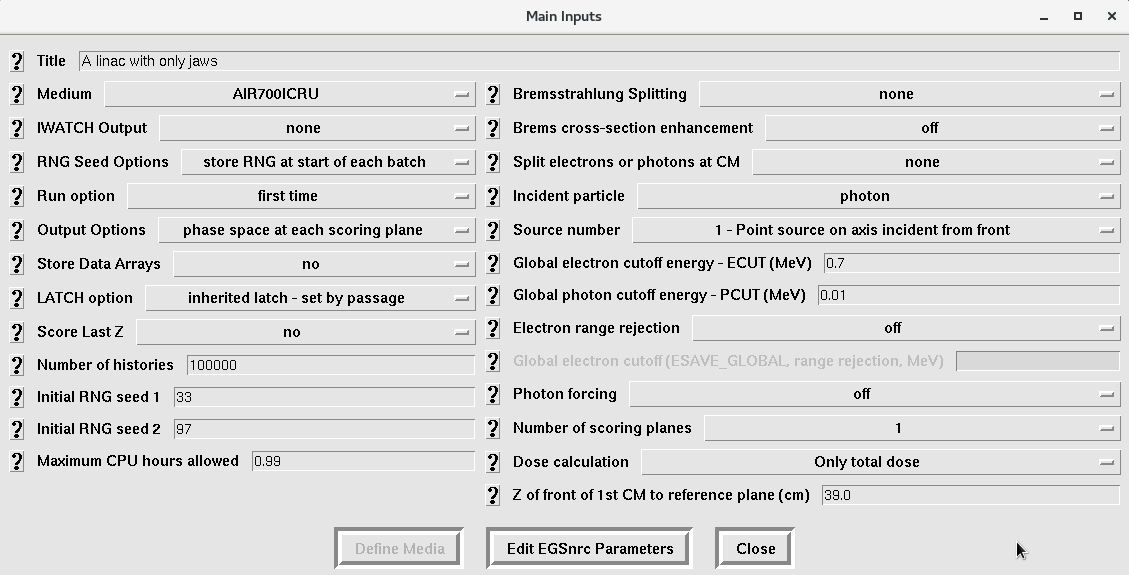
\includegraphics[width=6in]{figures/beamnrc_main}
\caption{BEAMnrc: Main input parameters}
\label{fig:beamnrc_mainInputs}
\end{center}
\end{figure}

\begin{figure}
\begin{center}
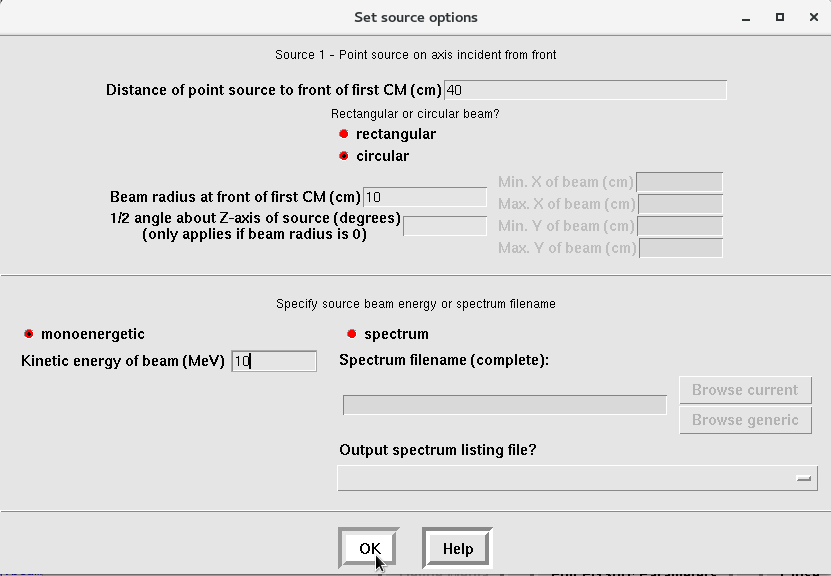
\includegraphics[width=5in]{figures/beamnrc_source1}
\caption{BEAMnrc: Source 1 options}
\label{fig:beamnrc_source1}
\end{center}
\end{figure}

\begin{figure}
\begin{center}
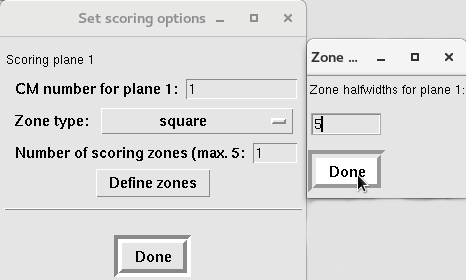
\includegraphics[width=3in]{figures/beamnrc_scoring}
\caption{BEAMnrc: Scoring options}
\label{fig:beamnrc_scoring}
\end{center}
\end{figure}

Close the main input parameters, and instead click the \,\Verb|Edit...|\, button next to \,\Verb|SYNCJAWS|\, to edit the input parameters for the jaws. Enter the parameters suggested in figure \ref{fig:beamnrc_syncjaws}, clicking the \,\Verb|Define jaw orientation/media|\, button to fill out the jaw settings. Set the \,\Verb|ECUT|\, and \,\Verb|PCUT|\, of the jaw material to 10~MeV. This is an approximation, but will greatly speed up the simulation for demonstration purposes.

For now, leave \,\Verb|File containing jaw opening data:|\, empty. We are setting up the component module (CM) for dynamic mode - motion of the jaws that can be synchronized with other components. Now would be a good time to save our progress \\
(\Verb|File -> Save input parameters as...|) giving the file a name like
\,\Verb|example.egsinp|\,.

\begin{figure}
\begin{center}
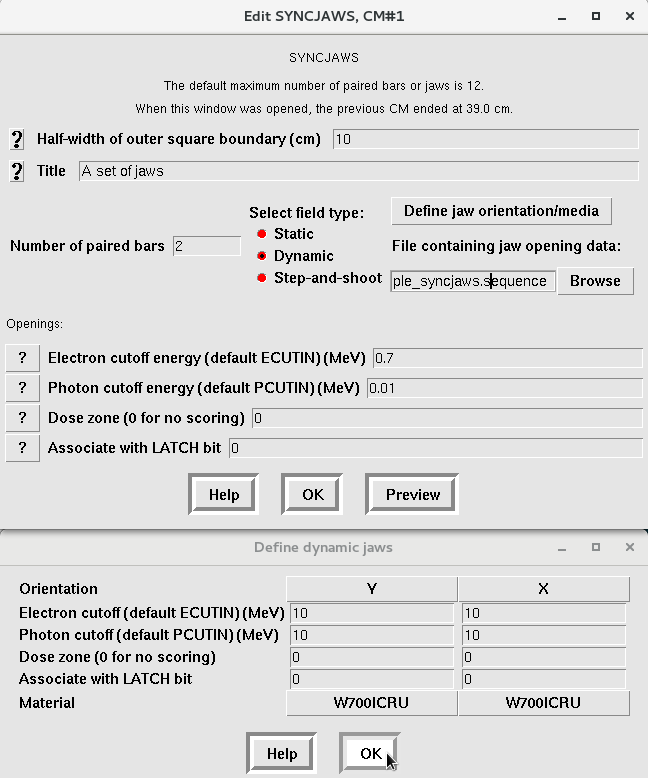
\includegraphics[width=5in]{figures/beamnrc_syncjaws}
\caption{BEAMnrc: Syncjaws definition}
\label{fig:beamnrc_syncjaws}
\end{center}
\end{figure}

Create a new text file, that will provide the dynamic motion of the jaws. There are examples for all of the syncronized CMs in \,\Verb|$HEN_HOUSE/omega/beamnrc/CMs/sample_sequences/|. Copy the text at the end of this section and save the file as \,\Verb|example.sequence|\, in \\
\,\Verb|$EGS_HOME/BEAM_syncjaws|\,. Now go back to the settings of the SYNCJAWS CM, click the \,\Verb|Browse|\, button and select the file (make sure the mode is set to \,\Verb|Dynamic|\,). Click \,\Verb|Preview|\, to view the first position of the jaws, before motion begins.

The format of the sequence file is described in section 15.3.8 of the BEAMnrc Users Manual (\href{https://nrc-cnrc.github.io/EGSnrc/doc/pirs509a-beamnrc.pdf}{PIRS509a}). Using this file, it is possible to model motion like jaw tracking, based on the \textit{index} parameter (i.e. fractional MU or cumulative meterset weight). If multiple SYNC CMs are included, the index is used to synchronize motion. Use a repeated index to simulate motion with the beam off.

In the following, we define 2 static fields and 1 dynamic field in 6 steps. The upper y-jaws are at $40 \le z \le 50$ and x-jaws at $51 \le z \le 61$. From index 0.0 to 3.0 (30\% of the simulation), the jaws are statically positioned. Similarly from 0.3 to 0.6. The repeated indices, 0.3 and 0.6, result in simulated collimator shifts while the beam is off. Finally, from index 0.6 to 1.0 (40\%) there is a motion of the x-jaws from a nearly-closed position to a $2 \times 2$ opening.

{\scriptsize
\begin{lstlisting}[language={},backgroundcolor=\color{white}]
Ex: 2 static fields, 1 dynamic, for 2 jaws
6
0.0
40, 50, -1, -1, -2, -2
51, 61, -1, -1, -2, -2
0.3
40, 50, -1, -1, -2, -2
51, 61, -1, -1, -2, -2
0.3
40, 50, 2, 2, 1, 1
51, 61, 2, 2, 1, 1
0.6
40, 50, 2, 2, 1, 1
51, 61, 2, 2, 1, 1
0.6
40, 50, 1, 1, -1, -1
51, 61, 0.05, 0.05, -0.05, -0.05
1.0
40, 50, 1, 1, -1, -1
51, 61, 1, 1, -1, -1
\end{lstlisting}
}

\subsection{Run a BEAMnrc simulation}
In the BEAMnrc GUI, go to \,\Verb|Execute -> Run|\, and click the \,\Verb|EXECUTE|\, button. Since we only set 100 histories to simulate, this will complete very quickly. Check the accelerator directory to find the phase-space that was saved as output \\
(\,\Verb|$EGS_HOME/BEAM_syncjaws/example.egsphsp1|\,). The 1 in \,\Verb|*.egsphsp1|\, refers to the scoring plane number of the phase-space (we scored after CM 1, but if you had more CMs you could score multiple phase-spaces in the same simulation). Additional output is recorded in the \,\Verb|*.egslst|\, file.

\clearpage
\subsection{Analyze the phase-space with beamdp}
Let's do a sanity check on the output of the BEAMnrc simulation by analyzing the phase-space using beamdp. Open the beamdp GUI. On linux this should be aliased:

\begin{lstlisting}
$ beamdp_gui
\end{lstlisting}

Perform a scatter plot of the phase-space to observe how the jaws have collimated the source (figure \ref{fig:beamdp_step1}). Suggested settings are shown in figure \ref{fig:beamdp_step2}, and the results in figure \ref{fig:beamdp_step3}. As expected, there are two off-axis fields, and one in the centre. Since the phase-space is scored immediately below the second set of jaws, it is easy to confirm that the field openings appear to match the collimator openings that were specified.

\begin{figure}
\begin{center}
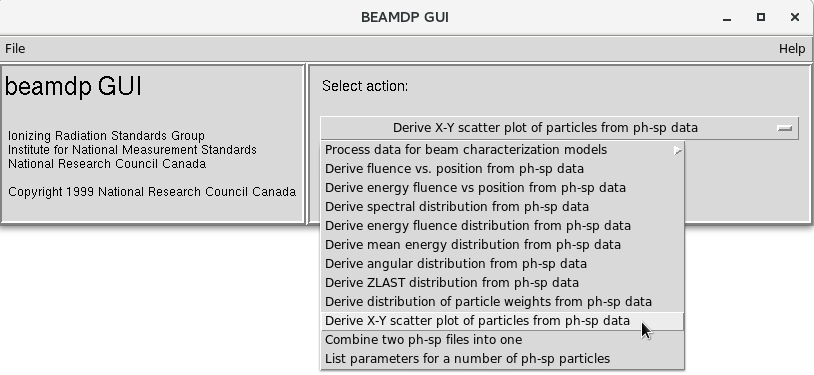
\includegraphics[width=5in]{figures/beamdp_step1}
\caption{BEAMDP: Mode selection}
\label{fig:beamdp_step1}
\end{center}
\end{figure}

\begin{figure}
\begin{center}
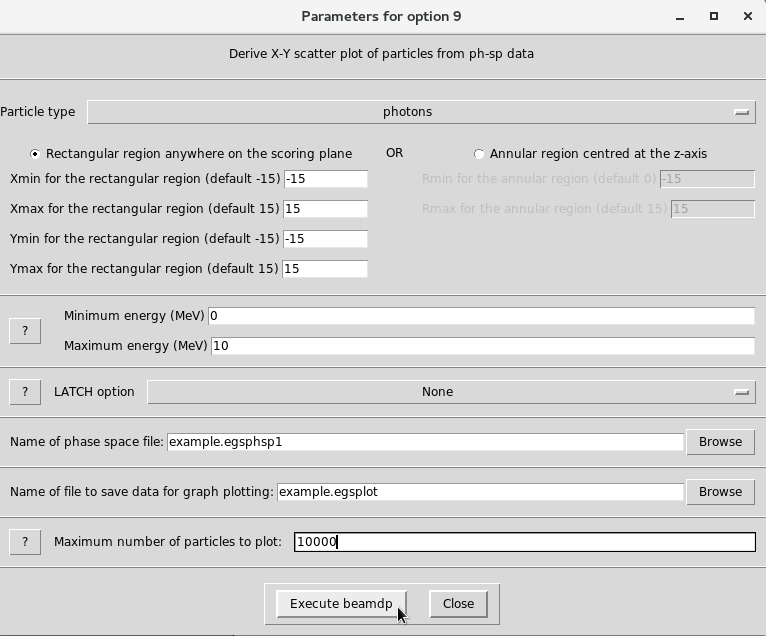
\includegraphics[width=5in]{figures/beamdp_step2}
\caption{BEAMDP: Plotting options}
\label{fig:beamdp_step2}
\end{center}
\end{figure}

\begin{figure}
\begin{center}
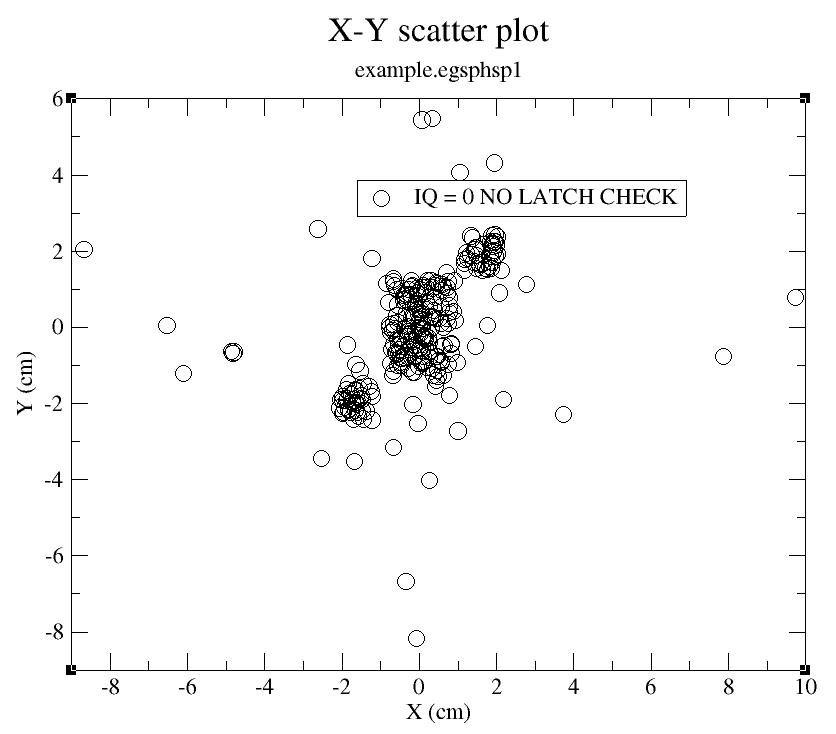
\includegraphics[width=3in]{figures/beamdp_step3}
\caption{BEAMDP: Example scatter plot}
\label{fig:beamdp_step3}
\end{center}
\end{figure}


\clearpage
\subsection{Convert CT DICOM data to egsphant}
In order to perform a MC simulation on a patient phantom, measured images need to be converted to the \,\Verb|egsphant|\, format. This is a rectilinear voxel format in a plain text file. There is a tool distributed with EGSnrc called \,\Verb|ctcreate|\, that can be used to convert CT DICOM files to the \,\Verb|egsphant|\, format.

A set of example CT DICOM files is provided in the \,\Verb|EGSnrc-sample-data.zip|\, file on the \href{https://github.com/nrc-cnrc/EGSnrc/releases}{release page}. Extract the zip file, and navigate to the \,\Verb|CT/DICOM|\, directory.

Edit the \,\Verb|CT_create_DICOM.inp|\, file so that the path to the \,\Verb|slice_files|\, file is correct (on line 2). Then open the \,\Verb|slice_files|\, file, and edit the paths to the ct files similarly. Also adjust the input parameters so that a higher resolution phantom is created. Note that this will use a default CT ramp that should be modified to agree with your imager (see the \,\Verb|ctcreate|\, section in the \href{https://nrc-cnrc.github.io/EGSnrc/doc/pirs794-dosxyznrc.pdf}{DOSXYZnrc Users Manual}).

{\scriptsize
\begin{lstlisting}[language={},backgroundcolor=\color{white}]
DICOM
/yourPath/EGSnrc-sample-data/CT/DICOM/slice_files
-150.0, 150.0, -150.0, 150.0, -45.0, 45.0
0.4, 0.4, 0.1
0,0
\end{lstlisting}
}

There is no GUI for \,\Verb|ctcreate|\,, so it has to be run from the command line (even on windows). From the directory containing the CT files, execute the command:

\begin{lstlisting}
$ ctcreate CT_create_DICOM.inp
\end{lstlisting}

This should create a new file in the directory, named \,\Verb|slice_names.egsphant|. Open this in a text editor to observe CT slices represented as 2D blocks of numbers. Each number corresponds to the material index (in the order they are listed at the top of the file). Following these blocks of integers are similar 2D blocks of floating point values - the density of each voxel. This format is described in the \href{https://nrc-cnrc.github.io/EGSnrc/doc/pirs794-dosxyznrc.pdf}{DOSXYZnrc Users Manual}.

Move the \,\Verb|egsphant|\, file into the \,\Verb|$EGS_HOME/dosxyznrc|\, directory for later use.

\clearpage
\subsection{Calculate dose with DOSXYZnrc}
The next task in the radiotherapy simulation process is to perform the dose calculation. To do this, create an input file for DOSXYZnrc and direct it to use a BEAMnrc source model and the \,\Verb|egsphant|\, file that was just created.

In order to use a BEAMnrc accelerator as a dynamic shared library source in DOSXYZnrc, the accelerator must be compiled as a shared library. This is an extra compilation step that is not performed by default. This must be done via command line (there is not an option to compile libraries in \,\Verb|egs_gui|\,). Navigate to the accelerator directory on the command line and type:

\begin{lstlisting}
$ make library
\end{lstlisting}

Open the DOSXYZnrc GUI, and start a new input file (figure \ref{fig:dosxyz_step1}). Make sure to select the same material data file that was used in BEAMnrc (i.e. \,\Verb|700icru|\, from the \,\Verb|HEN_HOUSE|\,).

\begin{lstlisting}
$ dosxyznrc_gui
\end{lstlisting}

\begin{figure}
\begin{center}
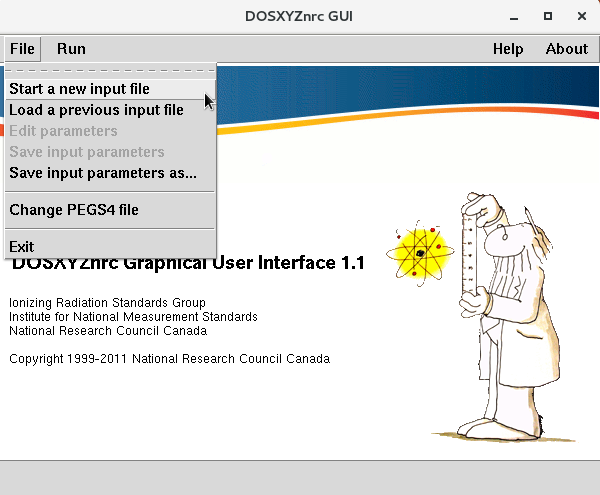
\includegraphics[width=4in]{figures/dosxyz_step1}
\caption{DOSXYZnrc: Start a new input file}
\label{fig:dosxyz_step1}
\end{center}
\end{figure}

Set the input parameters as shown in figure \ref{fig:dosxyz_step2}. Select source 21, which can be a dynamically synchronized source of particles from BEAMnrc. As long as the accelerator is compiled as a shared library, each particle that DOSXYZnrc needs will be requested from BEAMnrc. The accelerator model then simulates source particles until a particle reaches the scoring plane, at which point the DOSXYZnrc simulation can continue. Each particle is assigned a monitor unit value, to allow for the synchronization of time-dependent components. Notice that large values of \,\Verb|ECUT|\, and \,\Verb|PCUT|\, were chosen - this is just to speed up the simulation while we test parameters! If you would like an accurate simulation, reduce them to \,\Verb|ECUT=0.7|\, and \,\Verb|PCUT=0.01|\,.

\begin{figure}
\begin{center}
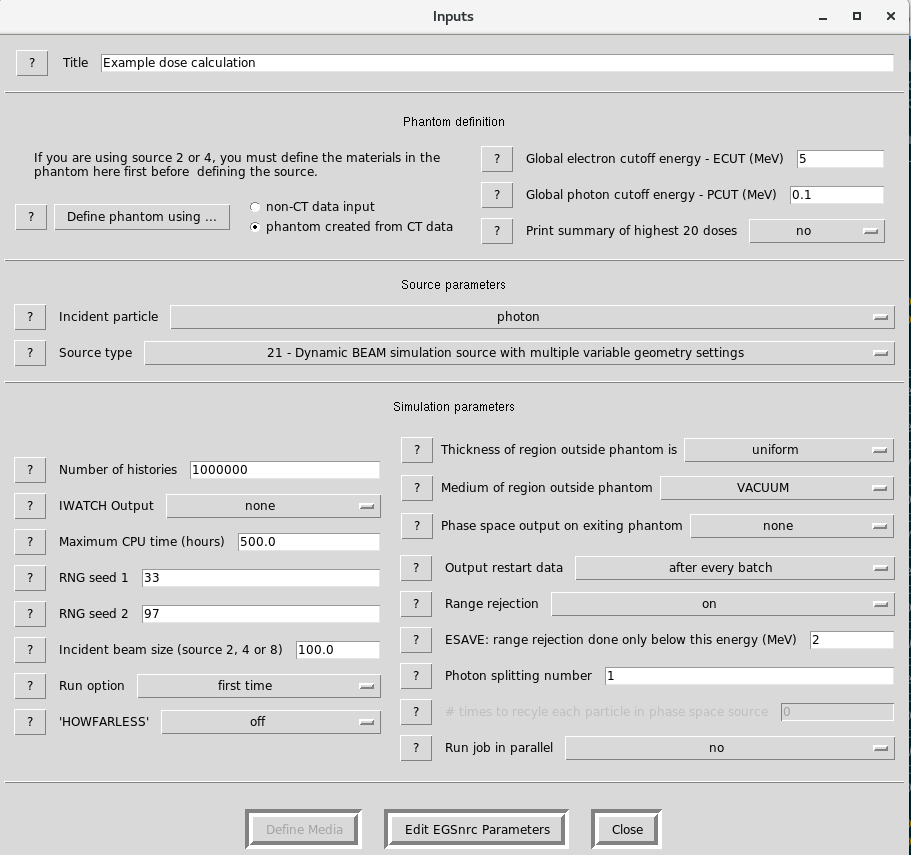
\includegraphics[width=5in]{figures/dosxyz_step2}
\caption{DOSXYZnrc: Set the main input parameters}
\label{fig:dosxyz_step2}
\end{center}
\end{figure}

\begin{figure}
\begin{center}
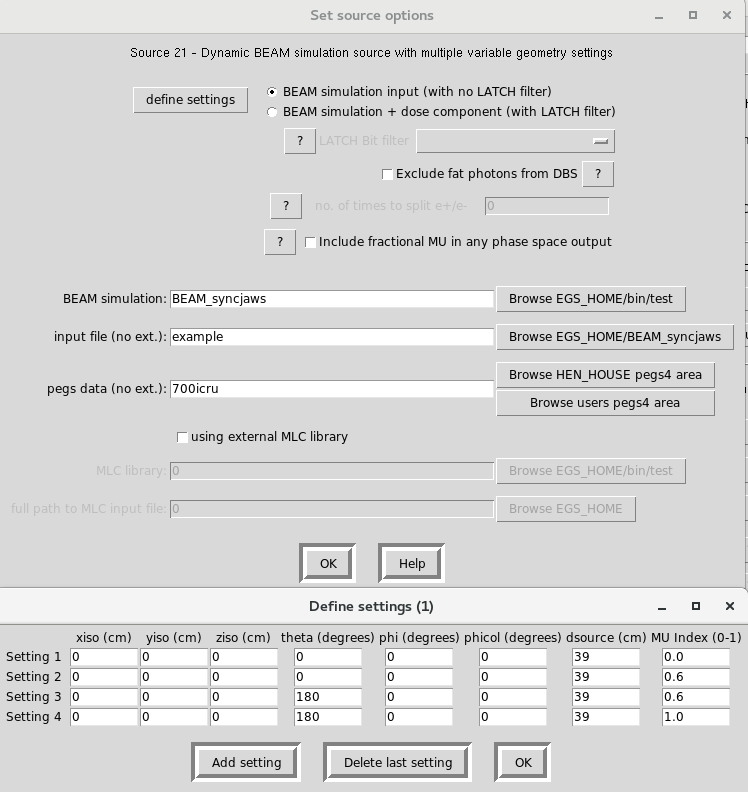
\includegraphics[width=5in]{figures/dosxyz_step3}
\caption{DOSXYZnrc: Set the synchronized source input parameters}
\label{fig:dosxyz_step3}
\end{center}
\end{figure}

For the synchronized source parameters, set two static source positions (later, play around with motion). From index 0.0 to 0.6, set the source to be incident along the negative z-axis. From 0.6 to 1.0, set the source to be incident along the positive z-axis.

Run the simulation! The output file of interest is the \,\Verb|example.3ddose|\,. file - this contains a 3D map of dose on the same grid as the \,\Verb|*.egsphant|\, file that we created from the CT data. To view the dose distribution, use the \,\Verb|dosxyz_show|\, tool.

\begin{lstlisting}
$ cd $EGS_HOME/dosxyznrc
$ dosxyz_show slice_files.egsphant example.3ddose
\end{lstlisting}

\begin{figure}
\begin{center}
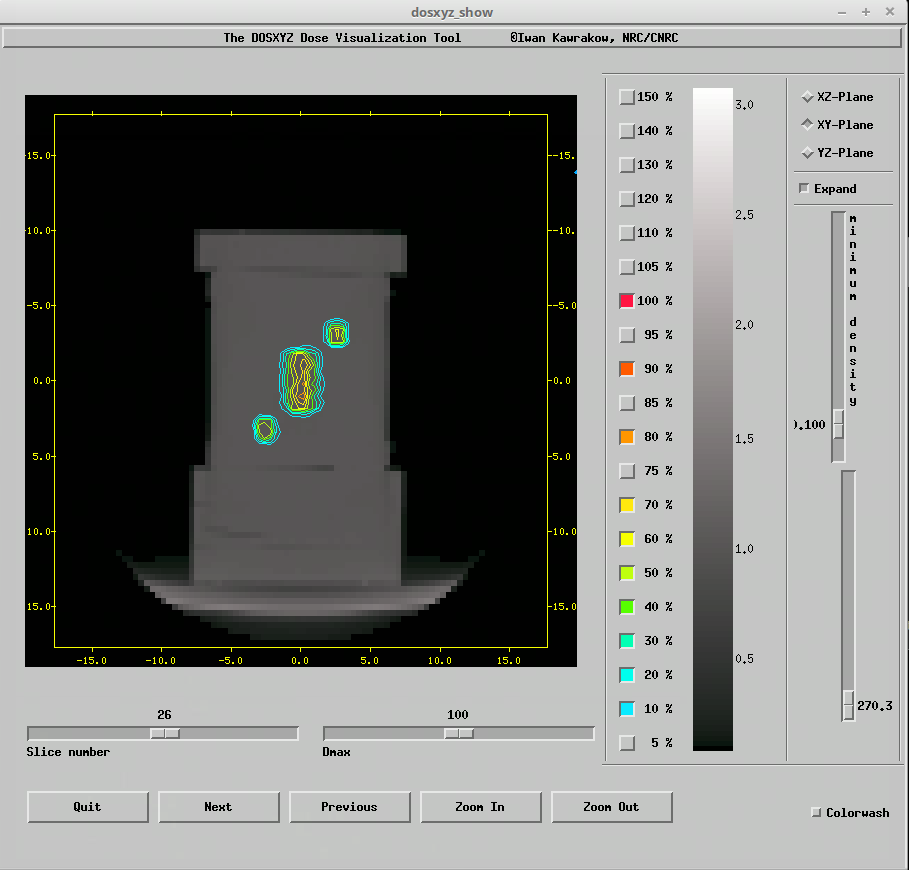
\includegraphics[width=5in]{figures/dosxyz_show}
\caption{dosxyz\_show: View the dose distribution}
\label{fig:dosxyz_show}
\end{center}
\end{figure}

\clearpage
\subsection{Extract dose profiles from 3ddose}
It is commonly of interest to obtain profile and depth-dose curves from dose files. For the 3ddose format, there is a tool distributed with EGSnrc that can do this called \,\Verb|statdose|\, (though many users design their own analysis software).

First, it may be necessary to adjust the \,\Verb|statdose|\, maximum array dimensions. Navigate to \,\Verb|$HEN_HOUSE/omega/progs/statdose|\, and open \,\Verb|statdose.mortran|\,. Change the \,\Verb|$MAXVOX|\, values to 300. The \,\Verb|$MAXVOXEL|\, parameter should be set to the maximum value of \,\Verb|$MAXVOXX|, \,\Verb|$MAXVOXY| and \,\Verb|$MAXVOXZ|. The save the file and recompile \,\Verb|statdose|\, (\,\Verb|make clean; make|\,).

{\scriptsize
\begin{lstlisting}[language={},backgroundcolor=\color{white}]
REPLACE {$MAXVOXX} WITH {200};
REPLACE {$MAXVOXY} WITH {200};
REPLACE {$MAXVOXZ} WITH {200};
REPLACE {$MAXVOXEL} WITH {200};
\end{lstlisting}
}

The \,\Verb|statdose|\, code does not have a GUI, so must be run from the command line. Navigate to \,\Verb|$EGS_HOME/dosxyznrc|\,, and type \,\Verb|statdose|\, to launch the program. This software uses text input - an example of both the output and input is shown below. Start with \,\Verb|Selection: 1|\, to read in dose distributions. In our directory we had 9 \,\Verb|*.3ddose|\, files listed, but you will probably just have one to choose. The number to the left of \,\Verb|example|\, is the file number to select (7 for us). Assign this file an internal reference number (use 1).

{\scriptsize
\begin{lstlisting}[language={},backgroundcolor=\color{white}]
*****************************************
        STATDOSE.MORTRAN
        Max array dimensions: 200 200 200
        Max # data sets: 15
*****************************************

 MAIN MENU
 --------
 0 - Exit
 1 - Read dose distributions
 2 - Statistical analysis
 3 - Normalization
 4 - Rebinning
 5 - Plot
 6 - Save

 Selection: 1

 READ DOSE DISTRIBUTIONS
 -----------------------
  1 16MVp_h2o_phantom_beamsource_example
  2 16MVp_h2o_phantom_phsp_example
  3 5MeV-2
  4 5MeV
  5 CT_example_electron
  6 edge_rot
  7 example
  8 tg195_test
  9 tg195_validation

 Input file number to Read in: (1- 9 or 0-Main Menu): 7
 File number for temporary storage: (1-* or 0-Main Menu): 1

 Number of voxels in X,Y,Z directions:         88        88        50
 Voxel-boundary values in X-direction:     -17.66  -  17.66
 Voxel-boundary values in Y-direction:     -17.66  -  17.66
 Voxel-boundary values in Z-direction:      -0.70  -   4.30
 Reading dose distribution...
 Reading in the uncertainties on DOSE Distribution...
\end{lstlisting}
}

After this, type 0 to return to the main menu, then select 5 to begin plotting. Plot profiles of 1 file, and select the x-axis to plot 3 curves at different y-positions. If you have xmgrace installed, it will launch automatically at this point to display the profiles. However, the data is also saved to the output file selected (e.g. \,\Verb|example.agr|\,). This is a plain text file, so even if you do not have xmgrace it is easy to load into a spreadsheet for data analysis and plotting.

{\scriptsize
\begin{lstlisting}[language={},backgroundcolor=\color{white}]
 Input file number to Read in: (1- 9 or 0-Main Menu): 0

 MAIN MENU
 --------
 0 - Exit
 1 - Read dose distributions
 2 - Statistical analysis
 3 - Normalization
 4 - Rebinning
 5 - Plot
 6 - Save

 Selection: 5

 PLOT MENU
 --------
 0 - Main menu
 1 - Plot profiles
 2 - Comparison plot

 Selection: 1

 Data for dose plot
 ------------------

 Files currently loaded
 ----------------------
 1 - example

 Number of file to Plot (0-PlotMenu): 1

 Axis for Profile (0-PlotMenu,1-X,2-Y,3-Z): 1
 Graph Title (default=Profile for example):
 Output Filename (default=example):
 Number of curves to Plot: 3
 Generate Automatic Offset? (y/n) [n]:

 Coordinates of Axis (y,z): 4,3

 3D-dose distribution  1: example
 Coordinates of Axis (y,z): 0,3

 3D-dose distribution  1: example
 Coordinates of Axis (y,z): -4,3

 3D-dose distribution  1: example

 Calling xmgrace...Please be patient!
\end{lstlisting}
}

If you have xmgrace installed, load the \,\Verb|*.agr|\, file later using the command:

\begin{lstlisting}
$ xmgrace example.agr
\end{lstlisting}

\clearpage
\section{Online resources}

\subsection{EGSnrc on github}

\begin{itemize}
\item EGSnrc can be downloaded (or ``cloned'') from the \Verb+github+ page. Make sure
to read the \href{https://github.com/nrc-cnrc/EGSnrc/wiki/Installation-overview}{installation instructions} carefully!

\href{https://github.com/nrc-cnrc/EGSnrc}{https://github.com/nrc-cnrc/EGSnrc}

\item The annual releases can be found on the github release page. Additionally,
pre-compiled GUIs, manuals and sample data are available:

\href{https://github.com/nrc-cnrc/EGSnrc/releases}{https://github.com/nrc-cnrc/EGSnrc/releases}

\item See the \Verb+wiki+ page for release notes, technical instructions and links to online documentation:

\href{https://github.com/nrc-cnrc/EGSnrc/wiki}{https://github.com/nrc-cnrc/EGSnrc/wiki}
\end{itemize}

\subsection{How to get support}
If you have a question, or encounter problems while using EGSnrc,
seek support on the EGSnrc reddit community! This is the best place
to get answers to questions ranging from the very simple to quite
complex. There are 200+ members who regularly answer questions, and
the EGSnrc developers also contribute frequently.

\href{https://www.reddit.com/r/EGSnrc/}{https://www.reddit.com/r/EGSnrc/}

To increase your chances of getting an answer, make sure to include as much information as possible in your original post. This should include:
\begin{itemize}
\item The EGSnrc application and version (e.g. \Verb+egs_chamber+, EGSnrc 2018 master branch)
\item Operating system
\item A clear description of the problem
\item Copy/pasted output including any errors
\item Optionally: compiler version, screenshots, input files and figures
\end{itemize}

\subsection{Bug reports}
Have you found a bug? Report it on the github \Verb+issues+ page! Make sure to include sufficient information for us to reproduce the bug.

\href{https://github.com/nrc-cnrc/EGSnrc/issues}{https://github.com/nrc-cnrc/EGSnrc/issues}

\subsection{Submitting your code}
Have you added a feature or fixed a bug? Submit the changes as a \Verb+pull request+! This requires learning the basics of ``git'' - if that is not feasible, you can also submit the changes as an \Verb+issue+ and allow one of us to create the pull request.

\href{https://github.com/nrc-cnrc/EGSnrc/pulls}{https://github.com/nrc-cnrc/EGSnrc/pulls}

\subsection{Documentation}
Documentation for EGSnrc is available online! However, keep in mind
that the documentation applies to the most recent \Verb+release+ of EGSnrc.
In other words, the documentation is generated annually, at the same time as the
release of the master branch (usually near the start of the year).

The online documentation:

\href{http://nrc-cnrc.github.io/EGSnrc/}{http://nrc-cnrc.github.io/EGSnrc/}

Each release is posted with the full set of manuals in a zip file. Find this on the release page:

\href{https://github.com/nrc-cnrc/EGSnrc/releases}{https://github.com/nrc-cnrc/EGSnrc/releases}

If you are using an older version of EGSnrc, or if you are working on the
\Verb+develop+ experimental branch, you may not find the matching documentation on the release page. To obtain the documentation that exactly matches your installation, find the documentation source code within your installation:

\Verb+$HEN_HOUSE/docs/src+

Some additional steps are required to compile the documentation locally.

\subsubsection{Compiling documentation locally}
\begin{enumerate}
\item Install a \latex suite that includes \Verb+pdflatex+, \Verb+bibtex+, \Verb+texmf+ and \Verb+makeindex+ (e.g. the \Verb+texlive+ suite includes all of these)
\item Install \Verb+doxygen+ (for the egs++ documentation)
\item \Verb+cd $HEN_HOUSE/docs/src+ (linux instructions)
\item \Verb+./makedoc.sh all+ (linux instructions)
\end{enumerate}

\clearpage
\section{EGSnrc file structure}
\begin{itemize}
\item \Verb+$HEN_HOUSE+: Points to location of the EGSnrc system (\textbf{user-defined})

\item \Verb+$EGS_HOME+: Points to user's working directory, where applications are copied (\textbf{user-defined})
\end{itemize}

\textbf{BEWARE:} Path to these folders cannot have spaces! EGSnrc relies on GNU \Verb+make+ which doesn't handle blank spaces in names. Also avoid special characters like $\&$.

\subsection{The \$HEN\_HOUSE}
The \Verb+$HEN_HOUSE+ directory contains all source code and data files for the
EGSnrc system. After installation, the contents of this directory generally remain unchanged.

\begin{table}[H]
\caption{The folder structure and contents of the HEN\_HOUSE.}
\begin{center}
\begin{tabular}{|p{0.2\linewidth}|p{0.15\linewidth}|p{0.6\linewidth}|}
\hline
% headers
Category & Folder & Description \\ \hhline{|===|}

% mortran & tcl code
\multirow{9}{*}{EGSnrc core} & \multirow{4}{*}{omega} & - BEAMnrc source code\\
    & & - addphsp, beamdp, ctcreate, dosxyz\_show, readphsp, and statdose \\
    & & - tcl GUIs for beamdp, BEAMnrc and DOSXYZnrc \\ \hhline{|~|-|-|}
    & \multirow{2}{*}{previewRZ} & - tcl GUI for viewing geometries from DOSRZnrc, CAVRZnrc, FLURZnrc and SPRRZnrc \\ \hhline{|~|-|-|}
    & src & - EGSnrc core MORTRAN source code \\ \hhline{|~|-|-|}
    & user\_codes & - Application source code (C++ and MORTRAN) \\ \hhline{|~|-|-|}
    & utils & - Various MORTRAN tools \\ \hhline{|===|}

% c++ & qt code
\multirow{6}{*}{egs++ and Qt} & cutils & - C tools for parallel jobs and BEAMnrc sources \\ \hhline{|~|-|-|}
    & \multirow{2}{*}{egs++} & - C++ class library \\
    & & - ausgab objects, geometries and sources \\ \hhline{|~|-|-|}
    & gui & - Qt GUIs: egs\_configure, egs\_gui and egs\_inprz \\ \hhline{|~|-|-|}
    & iaea\_phsp & - C++ tools for IAEA phase-spaces \\ \hhline{|~|-|-|}
    & interface & - The code that connects C++ and MORTRAN \\ \hhline{|===|}

% data
\multirow{9}{*}{data} & \multirow{4}{*}{data} & - photon cross section data \\
    & & - bremsstrahlung cross section corrections \\
    & & - eii cross sections \\
    & & - molecular form factors \\ \hhline{|~|-|-|}
    & \multirow{3}{*}{pegs4} & - PEGS4 mortran code \\
    & & - PEGS4 data files \\
    & & - density correction files \\ \hhline{|~|-|-|}
    & \multirow{2}{*}{spectra} & - various energy spectrum data \\
    & & - radionuclide decay data \\ \hhline{|===|}

% installation & supporting code
\multirow{5}{*}{configuration} & makefiles & - template application makefiles \\ \hhline{|~|-|-|}
    & mortran3 & - the MORTRAN core code \\ \hhline{|~|-|-|}
    & pieces & - system test code \\ \hhline{|~|-|-|}
    & scripts & - configuration and support scripts \\ \hhline{|~|-|-|}
    & specs & - configuration specifications \\ \hhline{|===|}

% documentation
documentation & docs & - documentation source code \\ \hhline{|===|}


\end{tabular}
\end{center}
\end{table}

Medium composition, electron stopping powers, and electron interaction cross sections, for media including with the EGSnrc distribution are contained in the \Verb+pegs4+ directory. The density correction files for \Verb+pegsless+ mode are found in \Verb+pegs4/density_corrections+ and the commonly used \Verb+521icru+ and \Verb+700icru+ pegs4 material data files are in \Verb+pegs4/data+.

There are a few example energy spectrum files contained in \Verb+spectra/egsnrc+. Radionuclide decay data in ensdf format for the egs++ radionuclide source are found in \Verb+spectra/lnhb+.

There are some scripts that help with configuration and parallel runs in \Verb+scripts+.

Compiled utility executables are found in \Verb+bin+, such as \Verb+ctcreate+, \Verb+beamdp+, etc.

\subsubsection{Configuring for different machines}

To compile EGSnrc on linux, there is a command line script that can be used instead of the installation GUI. This script is convenient to create different configurations that can be switched between - for example changing compile flags, or compiling for different machines.

\Verb+$HEN_HOUSE/scripts/configure+

The configure script does not create the \Verb+$EGS_HOME+ directory, unless you opt to run the \Verb+finalize_egs_foruser+ option at the end. Run the finalize script to create \Verb+$EGS_HOME+, copy over application source and compile applications (this would overwrite an existing \Verb+$EGS_HOME+). At the end of this script, the suggested environment variables are printed as output to the terminal (to be copy/pasted into your shell environment, such as \Verb+~/.bashrc+).

\Verb+$HEN_HOUSE/scripts/finalize_egs_foruser+

It is possible to have EGSnrc configured for execution on several servers, but sharing the same installation. This means that the configuration script is run once on each machine, and set to use a different configuration file (the \Verb+*.conf+ file) each time. To do this, watch for the prompt to set the configuration name and make sure to give it a unique identifier (usually the default is \Verb+linux.conf+). On each server, the \Verb+$EGS_CONFIG+ environment variable must be set uniquely, and should point to the main configuration file created by the installation script (but type it in as an absolute path, don't use environment variables):

\Verb+/full_path_to/HEN_HOUSE/specs/your_machine.conf+

On linux systems, the \Verb+$HEN_HOUSE+ and \Verb+$my_machine+ environment variables are automatically set using the \Verb+$EGS_CONFIG+ environment variable that you provide.

\subsection{The \$EGS\_HOME}
The \Verb+$EGS_HOME+ directory contains all of the applications and data created or provided by the user. Each application (previously called a \Verb+user_code+) has its own directory which contains the source code, a Makefile, and the user's input files. Output files from simulations are also written to the application directories.

The user may store their own set of material data in \Verb+$EGS_HOME/pegs4+, which will automatically supplement the data that is available in \Verb+$HEN_HOUSE/pegs4+.

\Verb+BEAMnrc+ has a folder structure different from other applications. Each accelerator that is built for \Verb+BEAMnrc+ is assigned its own directory with the name \Verb+BEAM_yourAccel+, where \Verb+yourAccel+ is the name of the accelerator. In other words, each accelerator is compiled as an independent EGSnrc application. The component module specifications for all accelerators are contained in \Verb+$EGS_HOME/beamnrc/spec_modules+.

The compiled executables for applications reside in \Verb+$EGS_HOME/bin/$my_machine+.

\begin{center}
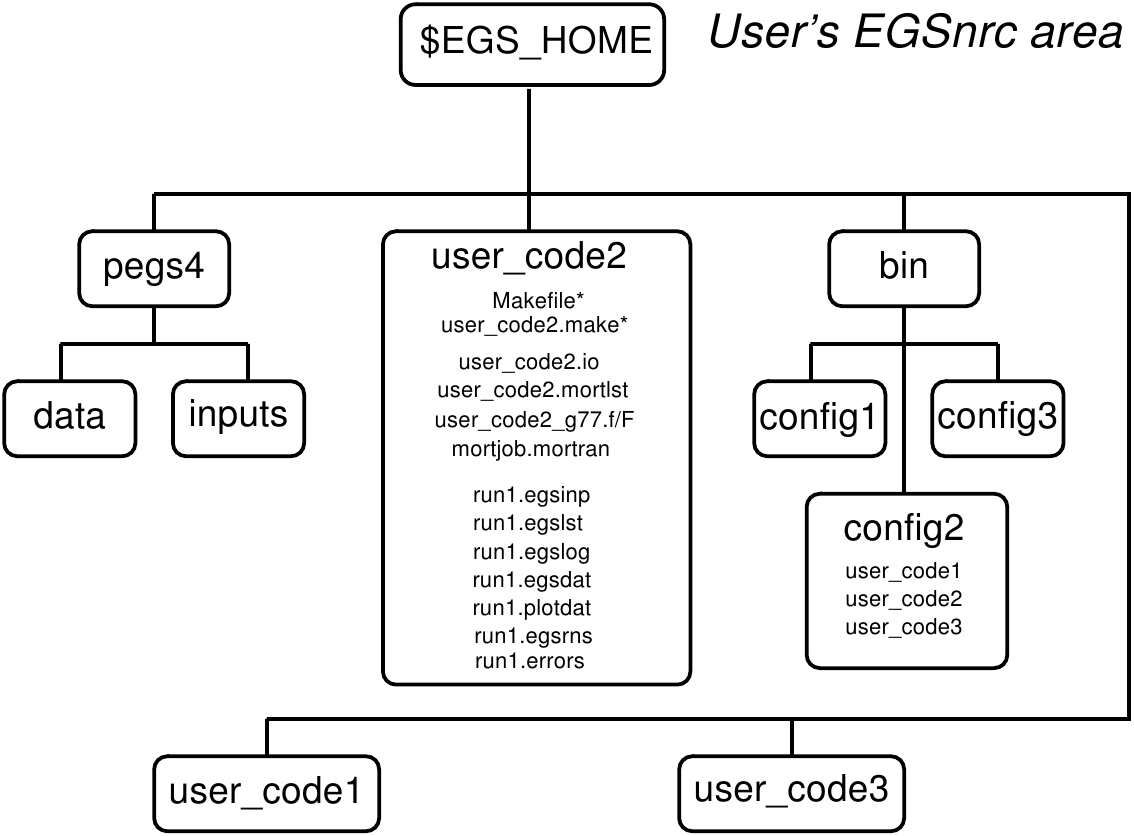
\includegraphics[width=5in]{figures/Users_EGSnrc_area}
\end{center}



% \section{References}
% \renewcommand{\rightmark}{References}
% \vspace*{-1cm}
% \setlength{\baselineskip}{0.5cm}
% \bibliography{../irs}
% \bibliographystyle{unsrt}

\end{document}
